\documentclass[../DC2019003Bouma.tex]{subfiles}
\begin{document}
\graphicspath{{03_Contribution/img/}}
\renewcommand{\chaptermark}[1]{\markboth{\thechapter.\ #1}{}}
\renewcommand{\sectionmark}[1]{\markright{#1}{}}

\pagestyle{fancyreport}
\cleartooddpage
\pagestyle{fancyreport}
\chapter{Sensitivity Analysis with Isolated State-and-Input-Triggered Events}\label{ch:order}
The behavior of trajectories tracking a nominal reference trajectory is analyzed in this chapter. More specifically, an analysis of tracking trajectories with state-and-input-triggered jumps of hybrid systems is presented. We will refer to the considered class of systems as \textit{nonlinear state-and-input-triggered hybrid systems} (NSITHS). In this chapter, isolated events are considered, indicating that guard functions are activated separately, such that there is always flow between the activations. The work in this chapter is an extension on \cite{Saccon2014,Rijnen2017,Rijnen2018a}, where a sensitivity analysis for \textit{nonlinear state-triggered hybrid systems} (NSTHS) has been presented. In this work, We will analyze the behavior of the system in the neighborhood of a nominal trajectory assuming that at least locally these isolated events also occur in the same sequence. However, the timing of the events will differ from the nominal event times for nearby trajectories. The mismatch in event time between the nominal trajectory and state trajectory can result in \textit{peaking behavior} of the tracking error \cite{Menini2001,Biemond2013}. Peaking behavior is known to result in undesirable large actuation forces. First, we introduce a different notion of error to avoid peaking behavior. After that, an approximation of the NSITHS will be presented in the form of a \textit{linear time-triggered hybrid system} (LTTHS), which we expect to be first order. There is no proof yet available that the LTTHS is a first-order approximation of the NSITHS, but it is strongly presumed. This chapter partially extends the work in \cite{Rijnen2017}, in the sense that the sensitivity analysis in this chapter is suitable for input-dependent guard functions, which are introduced by frictional effects and releasing motions. In \cite{Rijnen2017} there is also a proof which infers stability properties of an NSTHS about a reference trajectory from its corresponding LTTHS. Our claim is that a similar result will hold for the stability of the LTTHS implying local asymptotic stability of the NSITHS. This proof is however left for future work. Under the presumption that stability of the LTTHS implies local asymptotic stability of the NSITHS, conventional stability analysis tools for LTTHS can be used to asses the local stability of the NSITHS. Finally, a short summary of the findings in this chapter is given.
\nomenclature[A]{NSITHS}{Nonlinear State-and-Input-Triggered Hybrid System}%
\nomenclature[A]{LTTHS}{Linear Time-Triggered Hybrid System}%

\section{Trajectories with state-and-input-triggered jumps}
This section presents \textit{reference spreading} (RS) for trajectories with isolated events. Reference spreading is presented for isolated events in \cite{Saccon2014}, which is extended to be suitable for input-dependent guards in this section. When the hybrid system starts from a different initial condition than that of the reference trajectory for example, the resulting state trajectory and reference trajectory will likely have non-coinciding event-times. The notion of error defined in reference spreading eliminates the peaking behavior that results from the mismatch in event-time. In order to explain this notion of error better, we will first elaborate on the class of systems we consider, on the type of reference trajectories we allow, and we will introduce notation.
\nomenclature[A]{RS}{Reference Spreading}%

\subsection{Nonlinear state-and-input-triggered hybrid systems}
The framework of hybrid systems with impulsive effects is now used to formally define the NSITHS, which is the class of systems that is considered in this work.

\begin{sloppypar}
\begin{mydef}[NSITHS]\label{def:3nsiths}
A nonlinear state-and-input-triggered hybrid system is a system with dynamics of the form
\begin{align}
\dot{\xb}_j &=\fb_j(\xb_j,\ub_j,t), &\xb_j,\ub_j&\in \mathcal{C}_j\label{eq:3hybimp1}\\
\xb_{j+1} &= \gb_{j+1}(\xb_j,\ub_j,t), &\xb_j,\ub_j&\in \mathcal{D}_{j+1} \label{eq:3hybimp2}
\end{align}
with the state $\xb_j := \xb(t,j)$, the input $\ub_j := \ub(t,j)$, nonlinear vector field $\fb_j$, flow set $\mathcal{C}_j$ after event $j$, and a jump set $\mathcal{D}_{j+1}\subseteq\partial \mathcal{C}_j$, where when $(\xb_j,\ub_j)\in \mathcal{D}_{j+1}$ a state reinitialization is triggered according to the jump map $ \gb_{j+1}$ in \eqref{eq:3hybimp2}. Note that in $\xb_j$ and $\ub_j$, the time-dependency is implicit.
\end{mydef} 
\end{sloppypar}

Consider a nominal trajectory of an NSITHS, as illustrated in Figure~\ref{fig:3perturbedtraj} in red. We denote this nominal trajectory $\alphab_j:=\alphab(t,j)$ and assume it is the solution to \eqref{eq:3hybimp1}-\eqref{eq:3hybimp2} for input signal $\mub_j:=\mub(t,j)$ starting from initial condition $\alphab(t_0,0)=\alphab_0\in \mathcal{C}_0$. The following assumption on the nominal trajectory is imposed, to exclude that nominal jump times accumulate in time. Note that also for $\alphab_j$ and $\mub_j$, the time-dependency is left implicit.

\begin{sloppypar}
\begin{myass}[t-completeness and non-Zeno behavior of $\alphab$]
The reference trajectory $\alphab$ is defined for all $t>t_0$. Also, each segment $\alphab_j$ has non-vanishing time-domains $I^{\alphab}_j=[\tau_j,\tau_{j+1}]$, i.e., $\tau_{j+1}-\tau_j\geq c > 0$, where $\tau_j$ is the $j^{\textnormal{th}}$ event time and $c$ is a positive constant.\label{ass:nonzeno}
\end{myass}
\end{sloppypar}

\begin{sloppypar}
\begin{myremark}
The non-vanishing time-domains assumption posed in Assumption~\ref{ass:nonzeno} is guaranteed if $\gb_{j+1}(\alphab_j(\tau_{j+1}),\mub_j(\tau_{j+1}))\notin \mathcal{D}_{j+1}$ for all $j\in\{0,1,\dots,N\}$. This indicates that there is flow necessary, and therefore time, to reach the subsequent event set $\mathcal{D}_{j+1}$. 
\end{myremark}
\end{sloppypar}
Consider now a state trajectory $\xb$ starting from initial condition $\xb(t_0,0,\epsilon)=\xb_0(\epsilon)=\alphab_0+\epsilon \zb_0$ with input $\ub_j(\epsilon)=\mub_j+\epsilon \vb_j$, where $\epsilon$ is an initial state and input perturbation. In this $\zb_0 = \partial\xb_0 / \partial\epsilon$, $\mub_j = \mub(t,j)$ the feedforward corresponding to $\alphab_j$, and $\vb_j = \vb(t,j)$ the feedback. An example of a perturbed trajectory $\xb(\epsilon)$ is shown in Figure~\ref{fig:3perturbedtraj}.

\nomenclature[G05]{$\epsilon$}{The scalar perturbation parameter}%
\nomenclature[S05]{$(\cdot)^{\epsilon}$}{A variable dependent on the initial perturbation}%
\begin{figure}[bt!]
\centering
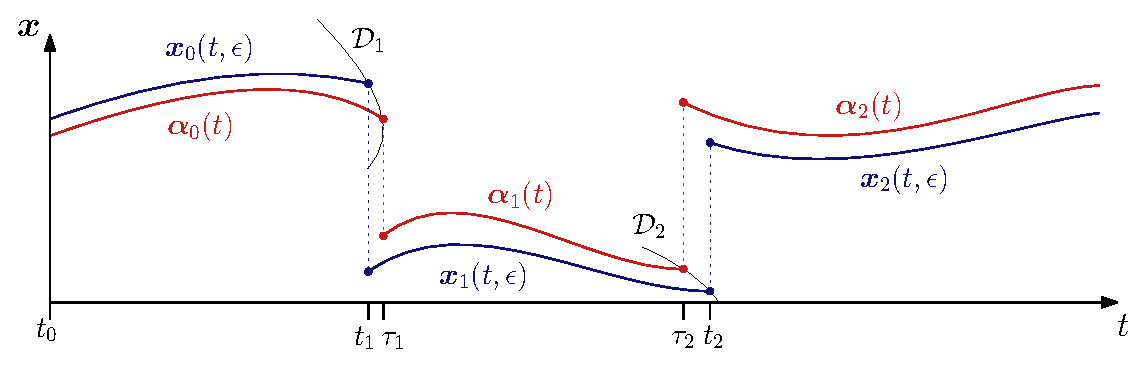
\includegraphics[width=.9\textwidth]{perturbedtraj.eps}\caption{A nominal (red) and a perturbed (blue) trajectory of a hybrid system with impulsive effects are depicted in this figure. The nominal and the state trajectory enter the jump sets $D$ at mismatching time instants, as a result from the perturbation in the state trajectory.} \label{fig:3perturbedtraj}
\end{figure}

For the nominal trajectory, the state and input curves are known over the entire time-domain, meaning that the event-times are also known. For the perturbed trajectory this is not the case. Referring to Figure~\ref{fig:3perturbedtraj}, there will be a mismatch between the nominal event times $\tau_1$ and $\tau_2$ and the perturbed event times $t_1$ and $t_2$. Taking a closer look at the first event of Figure~\ref{fig:3peakerror}, the peaking behavior can be illustrated as the result of a jump mismatch. In Figure~\ref{fig:3peakerror}, the state evolution $\xb$ of the first event is depicted besides the conventional tracking error $||\xb-\alphab||$ (assuming that $\alphab_j,\xb_j$ and $\alphab_{j+1},\xb_{j+1}$ are of the same dimension), where both trajectories are considered a function of conventional time $t$ alone. One can clearly see that a peak arises in the tracking error when the jump times do not coincide. At time equal to $t_1$, the state trajectory jumps, while the reference trajectory does not. At time equal to $\tau_1$, the reference trajectory jumps as well. This means that in $[t_1,\tau_1]$, a post-event state trajectory is compared to a ante-event reference trajectory, resulting in a large peak in the tracking error. This is undesirable in stability analysis and may for example lead to large and unnecessary actuation forces when considered in feedback control.

\begin{figure}[bt!]
\centering
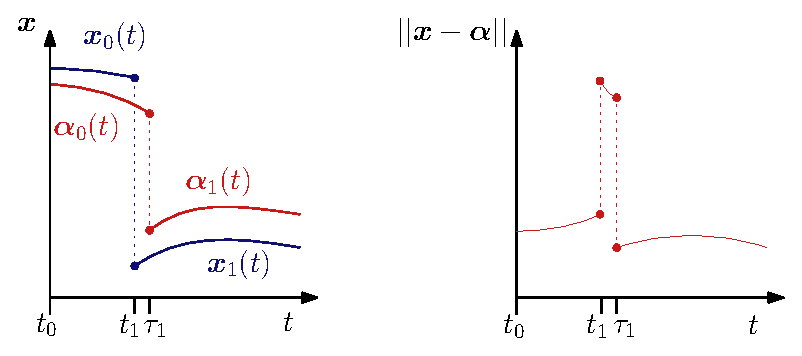
\includegraphics[width=.66\textwidth]{peakerror.eps}\caption{A closer look at the first event of the trajectory in Figure~\ref{fig:3perturbedtraj}. On the left the state-evolution $\xb$ is depicted and on the right the tracking error $||\xb-\alphab||$. A clear peak can be noticed in the tracking error as a result from the event-time mismatch.} \label{fig:3peakerror}
\end{figure}

In the next section, a different notion of error will be introduced that does not illustrate peaking behavior.
\nomenclature[G04]{$\Delta$}{The linearization of the perturbed event time around zero perturbation}%
\nomenclature[Ro]{$o(\cdot)$}{Landau's symbol little-o}%
\nomenclature[RG]{$\Gb$}{Positively homogeneous jump gain for the perturbed state direction}%
\nomenclature[RJ]{$\Jb$}{Positively homogeneous jump gain for the perturbed input direction}%
\nomenclature[RD]{$D_i(\cdot)$}{The derivative with respect to the $i$th term}%

\subsection{Reference-spreading}
To avoid peaking behavior in the tracking error, in \cite{Saccon2014} a methodology is presented which is named reference spreading in \cite{Rijnen2016}. In reference spreading a novel notion of error is introduced, called the \textit{reference spreading error} (RS error). The methodology uses reference trajectories which are extended beyond event-times, such that an ante-event state trajectory can always be compared to an ante-event reference trajectory and a post-event state trajectory can always be compared to a post-event reference trajectory. This is illustrated in Figure~\ref{fig:3refspread}, where the reference trajectory $\alphab_j$ is extended resulting in $\bar{\alphab}_j$. The extension is made by forward integrating the vector field $\fb_j$ beyond $\tau_{j+1}$ and backward integrating $\fb_j$ before $\tau_j$, for all $j\in\{0,1,\dots,N\}$. Adopting the notation of \cite{Goebel2009}, the hybrid domain of $\alphab$ is defined by segments $I_j^{\alphab} = [\tau_j,\tau_{j+1}]$, which together form the entire domain of $\alphab$ as
\begin{align}
\dom\alphab = \bigcup^N_{j=0}I^{\alphab}_j\times\{j\}.
\end{align}
\nomenclature[RI]{$I$}{Domain of a segment}%
Similarly the state segments $\xb_j$ are defined on the time intervals $I_j^\xb = [t_j,t_{j+1}]$ with the entire domain defined as
\begin{align}
\dom\xb = \bigcup^N_{j=0}I^{\xb}_j\times\{j\}.
\end{align}
The domain of the extended reference trajectory segments is extended such that $I^{\xb}_j\subseteq I^{\bar{\alphab}}_j$. The set of jump times of $\alphab_j$ and $\xb_j(\epsilon)$ are denoted as
\begin{align}
\text{eve}\ \alphab &= \bigcup_{j=1}^N \{\tau_j\}\times\{j-1\},\\
\text{eve}\ \xb &= \bigcup_{j=1}^N \{t_j\}\times\{j-1\},
\end{align}
respectively.
\begin{figure}[bt!]
\centering
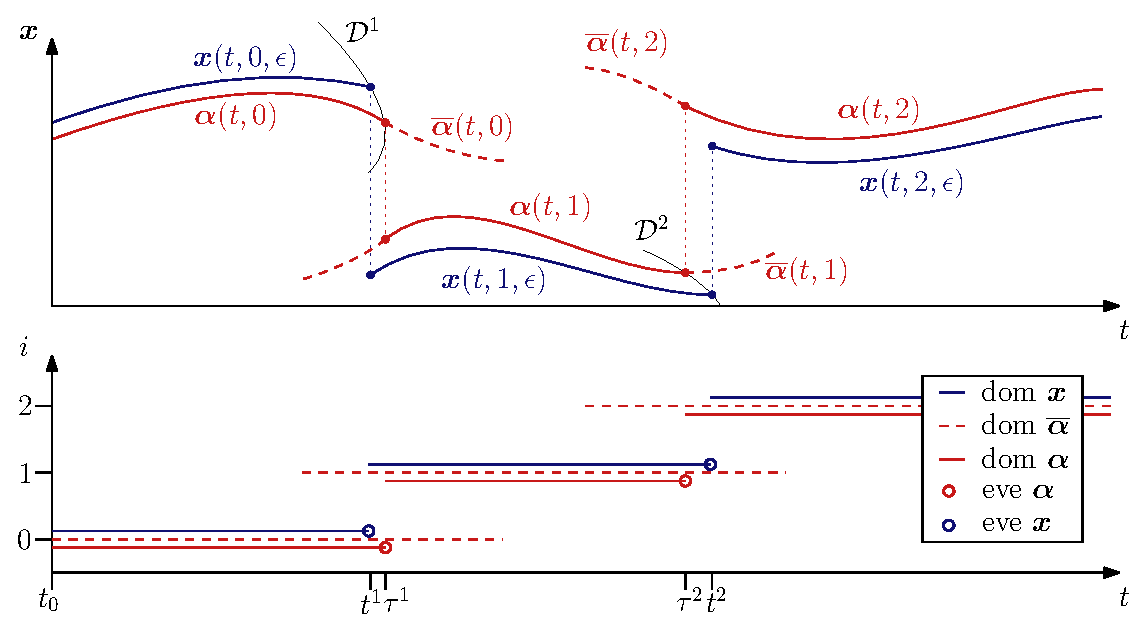
\includegraphics[width=.9\textwidth]{refspreaddom.eps}\caption{An illustration of the nominal reference trajectory (red) and the perturbed trajectory (blue), where the nominal reference trajectory is extended such that $\dom \xb\subseteq\dom \bar{\alphab}$.} \label{fig:3refspread}
\end{figure}

Let us now pose a continuity based assumption on the vector field $\fb_j$. This assumption (along with other assumptions) is instrumental to making sure that the ante-event state of the perturbed trajectory $\xb_j(t_{j+1},\epsilon)$ lies close to the ante-event state of the nominal trajectory $\alphab_j(\tau_{j+1})$, which is necessary to define an approximation of the perturbed trajectory.

\begin{sloppypar}
\begin{myass}[Lipschitz continuity of $\fb_j$]\label{ass:lipschitz}
We assume that in a neighborhood of the reference trajectory $\alphab_j$, $\fb_j$ is Lipschitz with respect to $\xb$ uniformly in $t$ and $j$. That is, $\exists\varepsilon_{\fb}>0$ and $\exists L$, independent of $t,j$, such that $\forall j$, $||\fb_j(\ab,t) - \fb_j(\bb,t)||<L||\ab-\bb||$, $\forall t\in (\tau_j - \varepsilon_{\fb},\tau_{j+1} + \varepsilon_{\fb})$ and $\forall \ab,\bb\in B_{\varepsilon_{\fb}}(\bar{\alphab}_j)$, where $B_{\varepsilon_{\fb}}(\bar{\alphab}_j)$ is a ball with radius $\epsilon_{\fb}$ around $\bar{\alphab}_j$.
\end{myass}
\end{sloppypar}

In the lower plot of Figure~\ref{fig:3refspread}, the hybrid time domains of $\xb$, $\alphab$ and $\bar{\alphab}$ are illustrated. Note that for every $j$, it holds that $I^{\xb}_j\subseteq I^{\bar{\alphab}}_j$. This means that the reference spreading error $||\xb-\bar{\alphab}||$ can be evaluated until $t=t_j$ is reached. The reference spreading error $||\xb-\bar{\alphab}||$ is therefore continuous for fixed $j$, even in the case where $t_j\neq\tau_j$, since the state $\xb_j$ will be compared to $\alphab_j$ until $t=t_j$ is reached. Once $t=t_j$, the counter $j$ is increased, and $\xb_{j+1}$ is compared to $\alphab_{j+1}$. Using this notion of error leaves only one jump at $t_j$ in the tracking error, even under the presence of event-time mismatches. More importantly, the peak in the tracking error is avoided, and an ante-event state trajectory will not be compared to a post-event reference trajectory (and vice versa) anymore. This is illustrated in Figure~\ref{fig:3refspreaderrors}, where the tracking errors with and without reference spreading are compared. Also, note that $\alphab_j$ and $\alphab_{j+1}$, for $j\in\{0,1,\dots,N\}$, do not need the be of the same dimension when the tracking error is defined as $||\xb-\bar{\alphab}||$.

\begin{figure}[bt!]
\centering
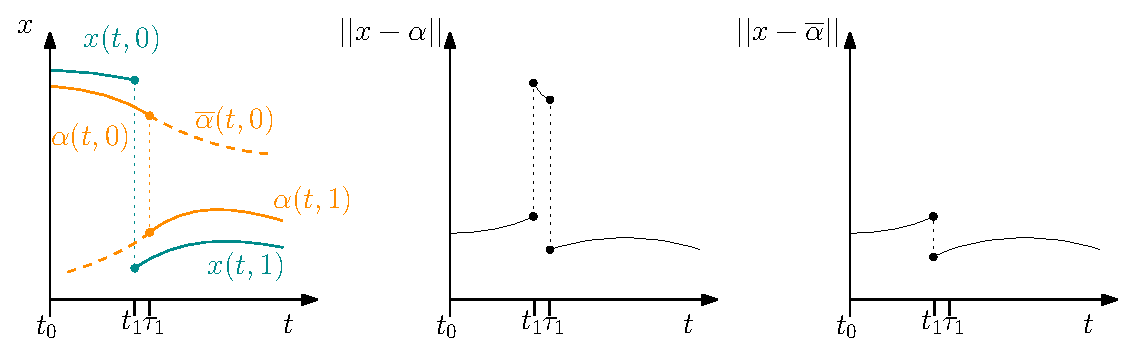
\includegraphics[width=\textwidth]{refspreaderrors.eps}\caption{A close up of the first event of the reference trajectory, with the conventional error $||\xb-\alphab||$ illustrated in the middle figure, and the reference spreading error $||\xb-\bar{\alphab}||$ in the right figure. Since $\bar{\alphab}$ is evaluated in the same mode as $\xb$, i.e., the reference spreading error is $||\xb_0 - \bar{\alphab}_0||$ for $t\leq t_1$ and $||\xb_1 - \bar{\alphab}_1||$ for $t\geq t_1$, the peaking behavior is not observed in the reference spreading error.}\label{fig:3refspreaderrors}
\end{figure}

In the next section, the reference spreading error will be used to analyze the behavior of perturbed trajectories with isolated events.

\section{Approximating perturbed trajectories with isolated events}\label{sec:3approx}
In \cite{Khalil1996} a sensitivity analysis is presented, where so-called sensitivity functions are used to provide first-order approximations of the effects of parameter variations on solutions. These sensitivity functions can also be used to approximate the solution under sufficiently small parameter variations. For the class of systems we consider here, the sensitivity equations describe the response of the system to perturbations in initial condition and input. This perturbation dynamics can be used to formulate an approximation of the perturbed state of the system, which we expect to be first-order. To find an approximation of state reinitializations in nonsmooth trajectories, an extension to this sensitivity analysis is necessary in the form of a linearized jump gain. The linearized jump gain and the linearized perturbation dynamics together define the LTTHS. In \cite{Rijnen2017} stability properties of an NSTHS are associated with the stability the corresponding LTTHS. In this section, the LTTHS is derived for an NSITHS, which we expect can be used to assess the stability of the NSITHS under the presumption that a similar relation between the LTTHS and NSITHS exists. As mentioned in the intro to this chapter, the proof for this relation is left as future work. For a more thorough derivation of the following analysis, Appendix~\ref{app:Csensitivity} should be consulted. We will first pose few assumptions on the reference events and jump maps that are required for the sensitivity analysis. First, we assume transversality of the reference events for which we assume the existence of a guard function that locally describes the flow and jump sets about each reference event.

\begin{sloppypar}
\begin{myass}[Existence of a guard function]\label{ass:existence}
We assume that there exist constants $\varepsilon_\gamma$, and real valued guard function $\gamma(\xb,\ub,t,j)$ which is continuously differentiable with respect to $\xb$, $\ub$, and $t$, for each $j\in \{1,2,\dots,N\}$, where $N$ is potentially infinite, such that
\begin{equation}
\begin{array}{llll}
\gamma_{j+1}(\xb_j,\ub_j,t) > 0 & &	&(\xb,\ub) \in B_{\varepsilon_\gamma}(\alphab_j(\tau),\mub_j(\tau))\cap \mathcal{C}_j\setminus\partial \mathcal{C}_j\\
\gamma_{j+1}(\xb_j,\ub_j,t) = 0 & &	&(\xb,\ub) \in B_{\varepsilon_\gamma}(\alphab_j(\tau),\mub_j(\tau))\cap \mathcal{D}_{j+1}\\
\gamma_{j+1}(\xb_j,\ub_j,t) < 0 & &	&(\xb,\ub) \in B_{\varepsilon_\gamma}(\alphab_j(\tau),\mub_j(\tau))\cap (\Rbb^n \times \Rbb^m \times \Rbb)\setminus \mathcal{C}_j
\end{array}
\end{equation}
where $B_{\varepsilon_\gamma}(\alphab_j(\tau),\mub_j(\tau))$ is a ball with radius $\varepsilon_{\gamma}$ around $\alphab_j(\tau),\mub_j(\tau)$ with $\tau = \tau_{j+1}$. The set $\mathcal{C}_j$ is the flow set of a trajectory after event $j$ and $\mathcal{D}_{j+1}\subseteq\partial \mathcal{C}_j$ is the event set which triggers event $j+1$, where $\partial \mathcal{C}_j$ represents the boundary of flow set $\mathcal{C}_j$. Note that $B_{\varepsilon_\gamma}(\alphab_j(\tau),\mub_j(\tau))\cap (\Rbb^n \times \Rbb^m \times \Rbb)\setminus \mathcal{C}_j$ only exists if $\mathcal{C}_j$ is not closed.
\end{myass}
\end{sloppypar}

\begin{sloppypar}
\begin{myass}[Transversal guard activations]\label{ass:transversality}
Under Assumption~\ref{ass:existence}, we assume there exists a constant $c>0$, such that
\begin{equation}
D_1\gamma_j(\alphab_j,\mub_j,t)\cdot\fb_j(\alphab_j,\mub_j,t) + D_2\gamma_j(\alphab_j,\mub_j,t)\cdot\fb_j(\alphab_j,\mub_j,t) + D_3\gamma_j(\alphab_j,\mub_j,t) \leq -c,
\end{equation}
for every event time $(t,j) \in \eve \alphab$.
\end{myass}
\end{sloppypar}

\begin{sloppypar}
\begin{myremark}
As can be seen in Assumption~\ref{ass:transversality}, the time derivative of the guard function at $\gamma_j(\alphab_j,\mub_j,t) = 0$ is needed to check for transversality. For $\gamma^{\text{sl}\rightarrow\text{st}} = \sqrt{\vbf_t^T\vbf_t}$, the time derivative is undefined when $\gamma^{\text{sl}\rightarrow\text{st}} = 0$. Therefore, a Taylor expansion is used to find the left limit of $\dot{\gamma}^{\text{sl}\rightarrow\text{st}}$ at $t = \tau_j$, to check whether the guard is activated transversally. More information on this can be found in Appendix~\ref{app:hybriddisc}.
\end{myremark}
\end{sloppypar}


%\begin{sloppypar}
%\begin{myass}[Isolated events]\label{ass:guardeventpair}
%With the set of all participating guard functions $\gamma^{\textnormal{part}}$, we assume that there exist a constant $\varepsilon_\gamma$, and set of nominal activated guard functions $\gamma^{\textnormal{nom}}_j$, such that
%\begin{align}
%\gamma^{\textnormal{part}}\setminus\gamma^{\textnormal{nom}}_j > 0,\quad \forall \xb,\ub\in B_{\varepsilon_\gamma}(\alphab(\tau,j),\mub(\tau,j),\tau),
%\end{align}
%where $\gamma_j = \gamma(\xb,\ub,t,j)$, and $B_{\varepsilon_\gamma}(\alphab(\tau,j),\mub(\tau,j),\tau)$ is a ball with radius $\varepsilon_{\gamma}$ centered around the ante-event state and input $\alphab(\tau,j),\mub(\tau,j)$ of event $j$.
%\end{myass}
%\end{sloppypar}

%Assumption~\ref{ass:guardeventpair} makes sure that the perturbed trajectory will activate the same guard functions as the reference trajectory.
The state, input and time where $\gamma_j(\xb_j,\ub_j,t) = 0$ represents the set where an event will happen, which together with Assumption~\ref{ass:transversality} guarantees that an event will happen, even under perturbations. If the vector field is continuous with respect to $\epsilon$, Assumption~\ref{ass:transversality} assumes that the vector field pushes the reference trajectory out of the flow set $\mathcal{C}_j$, and that grazing incidents are avoided. The combination of the existence of a guard function in an area around the nominal ante-event state and the transversal guard activation guarantees that there exists a range of perturbations where the guard is activated as well. Let us now pose an assumption on the jump map $\gb$.

\begin{sloppypar}
\begin{myass}[Locally differentiable jump maps]\label{ass:jump}
We assume that for all $j \in \{0,1,2,\dots,N\}$ the jump map $\gb_{j+1}(\xb_j,\ub_j)$ is locally differentiable, in the sense that $D_1\gb_{j+1}(\xb_j,\ub_j)$ and $D_2\gb_{j+1}(\xb_j,\ub_j)$ exist in the ball $B_{\varepsilon_{\gamma}}(\alphab_j(\tau),\mub_j(\tau),\tau)\subseteq \Rbb^n \times \Rbb^m \times \Rbb$, where $\tau = \tau_{j+1}$.
\end{myass}
\end{sloppypar}

The differentiability of the jump map is necessary to construct an approximation of the perturbed state trajectory. This will be explained in more detail in the next section.

\subsection{Sensitivity analysis}\label{sec:3sens}
The sensitivity analysis for the continuous segments of a perturbed trajectory gives a set of equations which describe the reaction of the system to an initial state-and-input perturbation. Introducing the initial state-and-input perturbation enables us to analyze the solution of a system under parameter variations. Writing \eqref{eq:3hybimp1} in integral form, a perturbed solution $\xb_j(t,\epsilon)$ to \eqref{eq:3hybimp1} satisfies
\begin{align}
\xb_j(t,\epsilon) = \xb_j(t_j,\epsilon) + \int_{t_j}^{t}\fb_j(\xb_j(s,\epsilon),\ub_j(s,\epsilon),s)ds.\label{eq:3xpert}
\end{align}
To find an approximation of the perturbed state, the perturbed state direction $\zb(t)$ and the perturbed input direction $\vb(t)$ are defined as
\begin{align}
\zb_j := \left.\frac{\partial\xb_j(\epsilon)}{\partial\epsilon}\right|_{\epsilon=0},\text{ and } \vb_j := \left.\frac{\partial\ub_j(\epsilon)}{\partial\epsilon}\right|_{\epsilon=0},\label{eq:3zbvb}
\end{align}
where we use the abbreviations $\zb_j = \zb(t,j)$, and $\vb_j = \vb(t,j)$. Conforming to the sensitivity analysis presented in \cite{Khalil1996}, a Taylor expansion is performed on $\xb_j(t,\epsilon)$ with respect to $\epsilon$. This results in
\begin{align}
\xb_j(t,\epsilon) &= \xb_j(t,0) + \epsilon\left.\frac{\partial\xb_j(t,\epsilon)}{\partial\epsilon}\right|_{\epsilon=0} + o(\epsilon).\label{eq:3taylor}
\end{align}
Since $\xb_j$ evaluated at $\epsilon=0$ is $\bar{\alphab}_j$, and using \eqref{eq:3zbvb}, we find
\begin{align}
\xb_j(t,\epsilon) &= \bar{\alphab}_j + \epsilon\bar{\zb}_j + o(\epsilon),\label{eq:3xbj}
\end{align}
with $o(\epsilon)$ indicating the Landau symbol little-o, which represents higher order terms $\epsilon$. The state perturbation $\zb_j$ in \eqref{eq:3xbj} is also extended, such that the approximation for $\xb_j$ can be extended beyond $I_j^{\alphab}$. To find an approximation of $\dot{\xb}_j(\epsilon)$, an expression for $\dot{\zb}_j$ should be found. By first taking the partial derivative of $\eqref{eq:3xpert}$ with respect to $\epsilon$, and then with respect to $t$, the perturbation dynamics are found to be
\begin{align}
\dot{\zb}_j = \Ab_j(t)\zb_j +\Bb_j(t)\vb_j,\label{eq:3zdot}
\end{align}
with
\begin{align}
\Ab_j(t) &= D_1\fb_j(\alphab_j,\mub_j,t),\\
\Bb_j(t) &= D_2\fb_j(\alphab_j,\mub_j,t),
\end{align}
where $D_a$ represents the partial derivative with respect to the $a$-th argument. By extending the perturbed input direction $\vb_j$, $\bar{\vb}_j$ is obtained. Using $\zb_0=\zb(0,\epsilon)$ and $\bar{\vb}_j$, $\dot{\zb}_j$ can be integrated past the nominal event-time $\tau_j$, which results in the extension of the perturbed state direction $\bar{\zb}_j$. With $\bar{\alphab}_j$ and $\bar{\zb}_j$, the first-order approximation of the perturbed state dynamics in continuous time can be defined as
\begin{align}
\dot{\xb}_j(\epsilon) = \dot{\bar{\alphab}}_j + \epsilon\dot{\bar{\zb}}_j + o(\epsilon).\label{eq:3contapprox}
\end{align}
Equation \eqref{eq:3contapprox} defines the first-order approximation for the continuous segments of a trajectory. What remains is that the state reinitializations should be linearized as well. The reinitialization of the nominal trajectory satisfies
\begin{align}
\alphab_{j}(\tau_{j}) = \gb_{j}(\alphab_{j-1}(\tau_{j}),\mub_{j-1}(\tau_{j}),\tau_{j}),\label{eq:3g}
\end{align}
and the reinitialization of the perturbed state is described by
\begin{align}
\xb_{j}(t_{j},\epsilon) = \gb_{j}(\xb_{j-1}(t_{j},\epsilon),\ub_{j-1}(t_{j},\epsilon),t_{j}).\label{eq:3gpert}
\end{align}
Similar to the Taylor expansion used in \eqref{eq:3taylor}, the state and input of the next segment evaluated at the perturbed event time $t_{j}$ can be expanded to
\begin{align}
\xb_j(t_{j},\epsilon) &= \bar{\alphab}_j(t_{j}) + \epsilon\bar{\zb}_j(t_{j}) + o(\epsilon),\label{eq:3xexpand}\\
\ub_j(t_{j},\epsilon) &= \bar{\mub}_j(t_{j}) + \epsilon\bar{\vb}_j(t_{j}) + o(\epsilon).\label{eq:3uexpand}
\end{align}
The same can be done for $\alphab_j(t_{j})$, $\mub_j(t_{j})$, $\zb_j(t_{j})$, and $\vb_j(t_{j})$, which also depend on $\epsilon$ since they are evaluated at the perturbed event time $t_j(\epsilon)$. Substituting these expansions in \eqref{eq:3xexpand} and \eqref{eq:3uexpand} results in
\begin{align}
\xb_j(t_{j},\epsilon) &= \alphab_j(\tau_j) + \epsilon\dot{\alphab}_j(\tau_j)\Delta + \epsilon\zb_j(\tau_j) + o(\epsilon),\label{eq:3xexpand2}\\
\ub_j(t_{j},\epsilon) &= \mub_j(\tau_j) + \epsilon\dot{\mub}_j(\tau_j)\Delta + \epsilon\vb_j(\tau_j) + o(\epsilon),\label{eq:3uexpand2}
\end{align}
with
\begin{align}
\Delta = \left.\frac{\textnormal{d} t_{j}}{\textnormal{d}\epsilon}\right|_{\epsilon=0}.\label{eq:3Delta}
\end{align}
To find $\Delta$, we observe that
\begin{align}
\gamma_j(\xb_{j-1}(t_{j},\epsilon),\ub_{j-1}(t_{j},\epsilon),t_{j}) = 0.\label{eq:3gamma}
\end{align}
Note that $\gamma_j$ is dependent on the input $\ub_j$, whereas in \cite{Chen2018a} the sensitivity analysis is performed for guard functions which solely depend on state $\xb_j$ and time $t$. From \eqref{eq:3gamma} the expression for $\Delta$ is found to be
\begin{align}
\Delta = -\frac{D_1\gamma^{-}\cdot\zb^- + D_2\gamma^{-}\cdot\vb^-}{\dot{\gamma}^{-}},\label{eq:3Deltaj}
\end{align}
with
\begin{align*}
\gamma^- &:= \gamma_j(\alphab_{j-1}(\tau_j),\mub_{j-1}(\tau_j),\tau_j),\\
\dot{\gamma}^- &:= D_1\gamma^-\cdot\dot{\alphab}_{j-1}(\tau_j) + D_2\gamma^-\cdot\dot{\mub}_{j-1}(\tau_j) + D_3\gamma^-,\\
\zb^- &:= \zb_{j-1}(\tau_j),\\
\vb^- &:= \vb_{j-1}(\tau_j),
\end{align*}
where the $(\cdot)^-$ superscript indicates a left limit of event $j$. Expanding the right-hand side of \eqref{eq:3gpert} gives
\begin{align}
\xb^+ &= \gb^- + \epsilon\left[\frac{\partial\gb_j}{\partial\epsilon}\right]_{\epsilon=0} + o(\epsilon),\\
&= \alphab^+ + \epsilon\left[\frac{\partial\gb_j}{\partial\xb}\left(\frac{\partial\xb^-}{\partial\epsilon} + \frac{\partial\xb^-}{\partial t}\frac{\text{d}t_j}{\text{d}\epsilon} \right) + \frac{\partial\gb_j}{\partial\ub}\left(\frac{\partial\ub^-}{\partial\epsilon} + \frac{\partial\ub^-}{\partial t}\frac{\text{d} t_j}{\text{d}\epsilon}\right) + \frac{\partial\gb_j}{\partial t}\frac{\text{d} t_j}{\text{d}\epsilon} \right]_{\epsilon = 0} + o(\epsilon),\\
&= \alphab^+ + \epsilon\left[D_1\gb^-\cdot \left(\zb^- + \dot{\alphab}^-\Delta\right) + D_2\gb^-\cdot \left(\vb^- + \dot{\mub}^- \Delta\right) + D_3\gb^-\cdot \Delta\right] + o(\epsilon),\label{eq:3gexp}
\end{align}
with
\begin{align*}
\xb^- &:= \xb_{j-1}(t_{j},\epsilon),\\
\xb^+ &:= \xb_{j}(t_{j},\epsilon),\\
\ub^- &:= \ub_{j-1}(t_{j},\epsilon),\\
\gb^- &:= \gb_j(\alphab^-,\mub^-,\tau_j),\\
\gb_j &:= \gb_j(\xb^-,\ub^-,t_j),\\
\alphab^- &:= \alphab_{j-1}(\tau_j),\\
\alphab^+ &:= \alphab_j(\tau_j),\\
\mub^- &:= \mub_{j-1}(\tau_j).
\end{align*}
Here, the $(\cdot)^+$ superscript indicates the right limit of event $j$. Rewriting \eqref{eq:3xexpand2} into
\begin{align}
\zb^+ &= \frac{1}{\epsilon}\left(\xb^{+} - \alphab^+\right) -\dot{\alphab}^+\Delta,\label{eq:3zexp}
\end{align}
with $\zb^+ := \zb_j(\tau_j)$ and substituting \eqref{eq:3gexp} into \eqref{eq:3zexp}, finally results in
\begin{equation}
\zb^+ = D_1\gb^-\cdot\left(\zb^- + \dot{\alphab}^-\Delta\right) + D_2\gb^-\cdot\left(\vb^- + \dot{\mub}^-\Delta\right) + D_3\gb^-\cdot\Delta - \dot{\alphab}^+\Delta,\label{eq:3zplus}
\end{equation}
By substituting \eqref{eq:3Delta} into \eqref{eq:3zplus}, we find
\begin{align}
\zb^+ = D_1\gb^-\cdot\zb^- + D_2\gb^-\cdot\vb^- - \left(D_1\gb^-\cdot \fb^- + D_2\gb^-\cdot\dot{\mub}^- + D_3\gb^-\cdot 1 - \fb^+\right)\frac{D_1\gamma^-\cdot\zb^- + D_2\gamma^-\cdot\vb^-}{\dot{\gamma}^-},
\end{align}
which can be rewritten in compact form as
\begin{align}
\zb^+ = \Gb_j(\tau_j)\zb^- + \Jb_j(\tau_j)\vb^-,\label{eq:3zbplus}
\end{align}
with 
\begin{align}
\Gb_j(\tau_j) & = D_1\gb^- - \left(\dot{\gb}^- - \fb^+\right)\frac{D_1\gamma^-}{\dot{\gamma}^-},\label{eq:3Gj}\\
\Jb_j(\tau_j) & = D_2\gb^- - \left(\dot{\gb}^- - \fb^+\right)\frac{D_2\gamma^-}{\dot{\gamma}^-},\label{eq:3Jj}
\end{align}
where
\begin{align*}
\fb^- &:= \fb_{j-1}(\alphab_{j-1}(\tau_j),\mub_{j-1}(\tau_j),\tau_j),\\
\fb^+ &:= \fb_j(\alphab_j(\tau_j),\mub_j(\tau_j),\tau_j),\\
\dot{\gb}^- &:= D_1\gb^-\cdot \fb^- + D_2\gb^-\cdot \dot{\mub}^- + D_3\gb^-.
\end{align*}
The jump gains in \eqref{eq:3Gj} and \eqref{eq:3Jj} consist of two terms. The first term in \eqref{eq:3Gj}, $D_1\gb^-$, represents the effect of the ante-event state perturbation on the post-event perturbation. The perturbation does not only change the ante-event state, but also the time-instant the event takes place. The second term in \eqref{eq:3Gj}, $- \left(\dot{\gb}^- - \fb^+\right)\frac{D_1\gamma^-}{\dot{\gamma}^-}$, represents the effect of the difference in time, in comparison to the nominal event. Obviously, the same can be said for \eqref{eq:3Jj}.

Equation \eqref{eq:3zbplus} describes the relation between the post-event state perturbation $\zb^+$ and the ante-event state and input perturbations $\zb^-$ and $\vb^-$. The relation given in \eqref{eq:3zbplus} is an extension on the results that have been obtained in \cite{Rijnen2018}. The jump gain in \cite{Rijnen2018} is derived with state-dependent guard functions $\gamma$ and jump gains $\gb$, whereas the jump gain $\Gb_j$ in \eqref{eq:3zbplus} is derived using state-and-input-dependent guard functions $\gamma$ and jump gains $\gb$. The second term in \eqref{eq:3zbplus} describes the effect of the ante-event input perturbation $\vb^-$ on the post-event state perturbation $\zb^+$, which is a contribution of this work. This term is a result of the jump gains $\gb$ being state-and-input-dependent, where in previous work the jump gains were considered state-dependent.

\subsection{Linear time-triggered hybrid system}
The sensitivity analysis performed in the previous section will be used next to define the LTTHS associated to reference trajectory $\alphab$ and the NSITHS defined in Definition~\ref{def:3nsiths}. The LTTHS converts the state-triggered behavior of the NSITHS to a time-triggered behavior using an approximation of the state jumps, which we expect to be first order. Where the jump times of the NSITHS are unknown, the LTTHS jumps at the same event-times as the nominal trajectory $\alphab$. Since the stability assessment of LTTHS is well established in literature, the LTTHS can then be used to conveniently assess the local asymptotic stability of the NSITHS. Let us now formally define the LTTHS.

\begin{sloppypar}
\begin{mydef}[LTTHS]\label{def:3ltths}
The linear time-triggered hybrid system associated with the reference trajectory $\alphab$ and the NSITHS \eqref{eq:3hybimp1}-\eqref{eq:3hybimp2} is given by
\begin{align}
\dot{\zb}_j &= \Ab_j(t)\zb_j + \Bb_j(t)\vb_j, &(t,j)&\in \dom\alphab,\\
\zb^+ &= \Gb_{j+1}(t)\zb^- + \Jb_{j+1}(t)\vb^-, &(t,j)&\in \eve\alphab,
\end{align}
with initial condition $\zb(t_0,0)=\zb_0$, $\zb^+ = \zb(t,j+1)$, $\zb^- = \zb(t,j)$,
\begin{align*}
\Ab_j(t) &= D_1\fb_j(\alphab_j(t),\mub_j(t),t),\\
\Bb_j(t) &= D_2\fb_j(\alphab_j(t),\mub_j(t),t),\\
\Gb_j &= D_1\gb^- - \left(\dot{\gb}^- - \fb^+\right)\frac{D_1\gamma^-}{\dot{\gamma}^-},\\
\Jb_j &= D_2\gb^- - \left(\dot{\gb}^- - \fb^+\right)\frac{D_2\gamma^-}{\dot{\gamma}^-},
\end{align*}
and
\begin{align*}
\dot{\mub}^- &:= \dot{\mub}_{j-1}(\tau_j),\\
\fb^- &:= \fb_{j-1}(\alphab_{j-1}(\tau_j),\mub_{j-1}(\tau_j),\tau_j),\\
\fb^+ &:= \fb_j(\alphab_j(\tau_j),\mub_j(\tau_j),\tau_j),\\
\gb^- &:= \gb_{j}(\alphab_{j-1}(\tau_j),\mub_{j-1}(\tau_j),\tau_j),\\
\dot{\gb}^- &:= D_1\gb^-\cdot \fb^- + D_2\gb^-\cdot \dot{\mub}^- + D_3\gb^-,\\
\gamma^- &:= \gamma_j(\alphab_{j-1}(\tau_j),\mub_{j-1}(\tau_j),\tau_j),\\
\dot{\gamma}^- &:= D_1\gamma^-\cdot\fb^- + D_2\gamma^-\cdot\dot{\mub}^- + D_3\gamma^-.
\end{align*}
\end{mydef}
\end{sloppypar}

The LTTHS of Definition~\ref{def:3ltths} gives an approximation of the NSITHS about the state-input reference trajectory $(\alphab,\mub)$. With a nominal trajectory $\alphab$ with input $\mub$, the perturbed trajectory $\xb_j(\epsilon)$ is the trajectory starting from initial condition $\xb_0(\epsilon) = \alphab_0 + \epsilon\zb_0$ and with input $\ub_j(\epsilon) = \mub_j + \epsilon\vb_j$. The approximation is then defined as $\xb_j(\epsilon) = \bar{\alphab}_j + \epsilon\bar{\zb}_j + o(\epsilon)$, with $\zb$ defined by the LTTHS. The reader should be aware that the term $\vb^-$ is not an input that can be freely chosen. The ante-event input perturbation $\vb^-$ is directly related to $\vb_j$, as it is a result of the input law implemented during the continuous segment before the event. Also, note that the approximation jumps at the same time instants as the nominal trajectory, with $(t,j) \in \eve\ \alphab$. This results in a trajectory which is generally infeasible around the jump times. However, due to the short timescales of the events, we are more interested in finding a good approximation of the continuous segments between the events, which is what the LTTHS achieves. In \cite{Rijnen2017} a proof is given, which shows that stability of the LTTHS implies tracking of a NSTHS. The presumption is made that a similar proof exists, saying that stability of the LTTHS implies local stability of the NSITHS.

\nomenclature[A]{NSTHS}{Nonlinear State-Triggered Hybrid System}%
\begin{figure}[bt!]
\centering
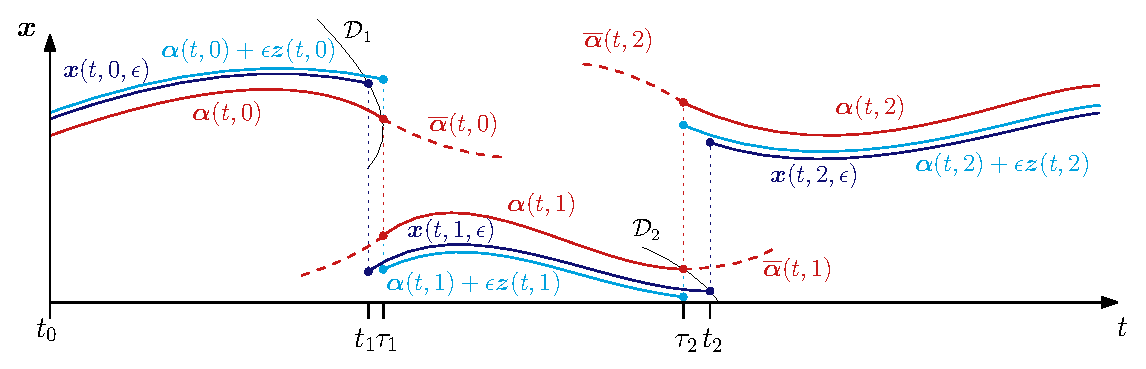
\includegraphics[width=\textwidth]{refspreadapprox.eps}\caption{The approximation of the perturbed trajectory $\alphab + \epsilon\zb$ (cyan) generated by the LTTHS is illustrated besides the perturbed trajectory $\xb$ (blue) and the nominal trajectory $\alphab$ (red). Note that the event times of the approximation are the same as those of the nominal trajectory.} \label{fig:3refspreadapprox}
\end{figure}

\section{Summary}
In this chapter, a linear approximation of the NSITHS is presented. The NSITHS is formally defined, which is a framework suitable for the dynamics defined in Chapter~\ref{ch:model}. Perturbations in the initial condition and input curve are introduced into this system, resulting in perturbed trajectories of which the event times differ from the nominal event times, and are not known beforehand. This mismatch in event time leads to a behavior called peaking. Reference spreading is then presented to eliminate peaking behavior. After posing assumptions on continuity of the vector fields, transversality of the guard activations, and differentiability of the jump maps, a sensitivity analysis is performed. The sensitivity analysis leads to an LTTHS describing the tracking error dynamics, which is used to generate an approximation of the perturbed state. While there is no proof available that the approximation generated by the LTTHS is first order, our claim is that such a proof exists. In addition, under the presumption that a proof exists that uniform asymptotic stability of the LTTHS implies local asymptotic stability of the NSITHS, conventional stability analysis tools can be used to evaluate tracking of the nominal reference trajectory.


%% new chapter %%
\cleartooddpage
\chapter{Sensitivity Analysis with Simultaneous State-and-Input-Triggered Events}\label{ch:simult}
\addtocontents{toc}{\vspace{\normalbaselineskip}}
In this chapter, the analysis presented in Chapter~\ref{ch:order} will be extended to be suitable for trajectories with simultaneous guard activations. Simultaneous guard activations are activations where a trajectory triggers two or more guard functions at the same time-instant. Take for example a box with two contact points, where both contacts are closed at the same time. When perturbations are introduced in these trajectories, the simultaneity of the event can be lost. Also, the order of activations can change depending on the perturbation. The box can first impact one contact point and then at the other, or the other way around. This complicates the definition of the approximation of the perturbed trajectory. 

In this chapter, a novel notation introduced in \cite{Rijnen2018} will be presented to describe trajectories with simultaneous guard functions. Reference spreading is applied to trajectories with simultaneous events, which is used as a basis to define a positively homogeneous jump gain which approximates the jump behavior of the perturbed trajectory. The positively homogeneous jump gain defines the \textit{positively homogeneous time-triggered hybrid system} (PTTHS). This chapter extends the work presented in \cite{Rijnen2018,Rijnen2018a}, making the approximation suitable for trajectories with input-dependent guard functions, and therefore mechanical systems experiencing dry friction and releasing motions.

\section{Simultaneous guard-activation}\label{sec:simguards}
To be able to perform a sensitivity analysis in the spirit of the one presented in Chapter~\ref{ch:order} for trajectories with simultaneous guard activations, some adjustments need to be made to the notation of the system definition. In this section, a notation similar to the notation in \cite{Rijnen2018} is presented, namely: the event character, micro and macro events, multiscale hybrid time, guard function index, mode descriptor, phantom segments, and historical notation. After this, reference spreading for simultaneous guard-activations is discussed. Note that the notation that will be presented in this section is not a contribution, but merely presented for completeness.

\subsection{Adopted notation}\label{sec:4not}
In a simultaneous event, multiple guard functions are activated at the same time instant. In Figure~\ref{fig:4simulexample}, an example of a simultaneous activation of two guards is illustrated. The ante-event reference trajectory, $\alphab_0(t)$, activates two guard functions, $\gamma_1$ and $\gamma_2$. The number of guard functions that are activated in a single nominal event is called the \textit{event character}, and indicated with the letter $c$. In the example in Figure~\ref{fig:4simulexample}, the event character is two $(c = 2)$.

\begin{figure}[bt!]
\centering
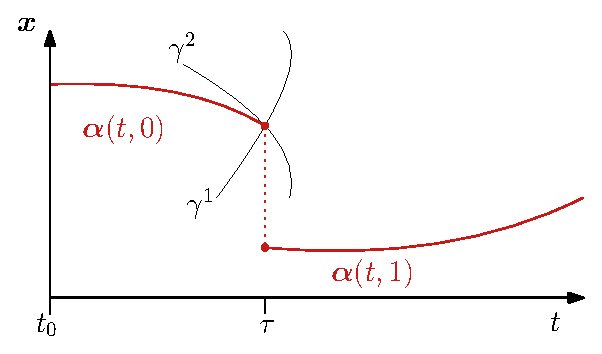
\includegraphics[width=.45\textwidth]{simulexample.eps}\caption{An illustration of a trajectory with a simultaneous event. At $t=\tau$, the trajectory activates two guard functions, $\gamma_1$ and $\gamma_2$.} \label{fig:4simulexample}
\end{figure}

When perturbations are introduced in an event with simultaneous activations, the number of events the system undergoes can change. Instead of a simultaneous activation of $c$ guards, the guards can be activated in rapid succession. These events that are the result of loss of simultaneity are called \textit{micro events}, where several micro events are associated to the same transition. Such a transition is called a \textit{macro event}. When a macro event consists of simultaneous activations, one jump will be observed. Loss of simultaneity will generate micro events, resulting in that more jumps and flow segments can be observed in the state trajectory in comparison to the reference trajectory. To keep track of these segments, \textit{multiscale hybrid time} is introduced. Multiscale hybrid time is denoted by $(t,i,k)$, where $t$ is regular time, $i$ the macro event counter, and $k$ the micro event counter. The micro event counter $k$ is incremented every time an event occurs, except when a macro event is completed by reaching the nominal post-event mode. The micro event counter $k$ is then reset to zero, and the macro event counter $i$ is incremented. One can now write $\xb(t,i,k)$ to make a distinction between all the segments that are generated as a result of loss of simultaneity. Multiscale hybrid time is directly related to the standard hybrid time as defined in Section~\ref{sec:2hyb}, according to
\begin{align}
j(i,k) = k + \sum_{\kappa=1}^{i}l_\kappa,
\end{align}
with $l_\kappa$ the number of micro events in macro event $\kappa$. The perturbed event times of micro events are denoted by $t^k_i$, i.e., the event time of the $k$-th micro event of macro event $i$. A set of guard function indexes $\eta$ is introduced to identify the several guard functions that are involved with an event. A guard function that is inactive is a guard function that is associated to a transition, but not yet activated. With $c_i$ the event character of the $i$-th event, the index set of inactive guard functions is defined as
\begin{align}
\big\{\eta = 2^{\nu}\ |\ \nu\in\{0,1,\dots,c_i\}\big\}.\label{eq:4eta}
\end{align}
The index set of inactive guard functions $\eta$ is written in the binary numeral system for a more intuitive notation of the different guard functions. The inactive guard functions can then be denoted as $\gamma^\eta$. While the micro counter $i$ and macro counter $k$ are left out for readability, note that
\begin{align}
\gamma^\eta = \gamma^\eta(\cdot,i,k),\label{eq:4gammaik}
\end{align}
meaning that the guard functions not only change with macro events, but also with micro events. Now an example is given to illustrate the relation between the set of guard functions $\gamma^\eta$ and the guard functions defined in Section~\ref{sec:2event}. Let us consider a block with two contact points not in contact, i.e., $\iota_1,\iota_2\in\mathcal{I}_{\text{op}}$. We consider a nominal trajectory with a character-2 event ($c=2$), where both contact points simultaneously close contact with a surface. The index set of inactive guards $\eta$ before the event is, in this example, $\eta = \{01,10\}$. The associated guard functions are then defined as
\begin{align}
\gamma^{01} &= \gamma^{\text{op}\rightarrow\text{cl}}_{\iota_1} = \hrm_{n,\iota_1}(\qb),\\
\gamma^{10} &= \gamma^{\text{op}\rightarrow\text{cl}}_{\iota_2} = \hrm_{n,\iota_2}(\qb).
\end{align}
The mode of the system is indicated using the \textit{mode descriptor} $s^k_i$. The mode descriptor $s^k_i$ is associated to event $i$, similar to $\tau_i$\footnote{The reader should be aware of the distinction between the event $i$ and the hybrid time $i$. The hybrid time $i$ indicates a segment of flow, whereas the event $i$ indicates a point.}. The micro segments associated to macro event $i$ will be described using
\begin{align}
\ls^{s^k_i}\xb(t) := \xb(t,i-1,k),
\end{align}
with $s^k_i$ the mode of the $k$-th micro event associated to macro event $i$. Note that $s_i^k$ is a mode descriptor to describe the micro segments associated to macro event $i$. The macro segments, where $k=0$, are still written as 
\begin{align}
\xb_i(t) = \xb(t,i,0).
\end{align}
When the considered macro event is known from context, the macro counter $i$ can be dropped to simplify the notation. From here on, we will also write the mode descriptor as $s^k$ if the macro counter $i$ is known. Similar to the inactive guard index set $\eta$, the mode descriptor is written in the binary numeral system. This binary numeral system is used as follows. When there is an event with character $c = 4$, four guard functions can be activated. When the mode of the system is described by $s^k = 1010$, this means that two guard functions are already activated, and two are still inactive. Namely, the guard functions that are still to be activated are those with index $\eta = \{0100,0001\}$. The mode descriptor now intuitively shows which guard functions are inactive, as the zeros in the mode descriptor denote the inactive guard function indexes. The index of the guard function that is activated during event $k$ is denoted by $\eta_k$. The superscript $(\cdot)^{\epsilon}$ is introduced for the state $\xb$, to indicate that the state trajectory is perturbed, i.e.,

\begin{align}
\ls^{s^k_i}\xb^{\epsilon}(t) = \xb(t,i-1,k,\epsilon).
\end{align}

We will illustrate the adopted notation in an example. Let us consider a transition, depicted in Figure~\ref{fig:4simulpert}, with event character $c = 2$ and guard functions $\gamma^{10}$ and $\gamma^{01}$. The state evolution of the system begins in the mode described by $s^0 = 00$, where $\gamma^{10}>0$ and $\gamma^{01}>0$. When the state activates one of the guard functions, in the example of Figure~\ref{fig:4simulpert} $\gamma^{01}=0$, the next mode is described by $s^1 = 01$. When the other guard function $\gamma^{10}$ is activated as well, then the system completes its macro event with $s^2 = 11$. Note that the guard function can change when the system is in another mode, i.e., the guard function $\gamma^{10}$ defined in $s^0$ is different from the guard function $\gamma^{10}$ defined in $s^1$.

\begin{figure}[bt!]
\centering
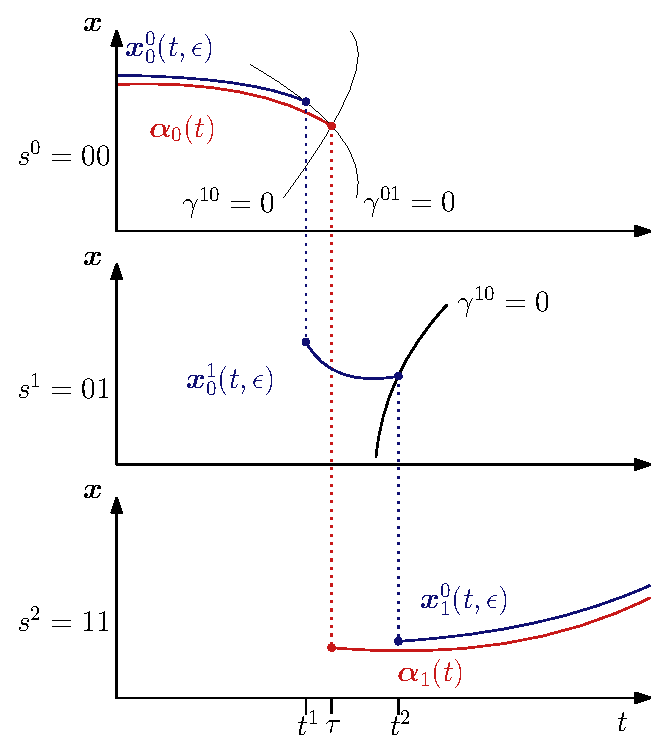
\includegraphics[width=.52\textwidth]{simulpert.eps}\caption{A reference trajectory going through a simultaneous event and a state trajectory experiencing loss of simultaneity. Where the reference trajectory activates $\gamma^{10}$ and $\gamma^{01}$ simultaneously, the state trajectory first activates $\gamma^{01}$ at $t=t^1$, flows for $t\in [t^1_1,t^2_1]$, and then activates $\gamma^{10}$ at $t=t^2$.}\label{fig:4simulpert}
\end{figure}

Depending on the perturbation, several mode sequences can achieve the expected nominal end mode when simultaneity is lost. The different mode sequences can generate a different post-event state, because of the flow phases in between the micro events. Therefore, it is useful to be able to indicate an entire mode sequence with one symbol. We call this notation the \textit{historical notation}. We define the sequence for macro event $i$ as 
\begin{align}
S^k_i = s^k_i\leftarrow s^{k-1}_i\leftarrow \dots \leftarrow s^0_i,
\end{align}
where $s^0_i = 00\dots0$ with length $c_i$. Again, the macro counter $i$ can be left out for convenience. A growing mode sequence is a sequence of micro events, where at each micro event another guard function is activated and no guard functions deactivated. We can now define $\ls^{S^k}\xb(t)$ as $\ls^{s^k}\xb(t)$ that is a result of the growing sequence $S^k$. The jump maps that are applied during such a sequence are given by
\begin{align}
\ls^{p}\xb = \ls^{p\leftarrow a}\gb(\ls^{a}\xb,\ls^{a}\ub,t),
\end{align}
where $p$ represents the post-event mode descriptor, and $a$ the ante-event mode descriptor. For example, the state jump from $s^k$ to $s^{k+1}$ is given by $\ls^{s^{k+1}}\xb = \ls^{s^{k+1}\leftarrow s^k}\gb(\ls^{s^k}\xb,\ls^{s^k}\ub,t)$. Sequences with a particular order of events can also be expressed as
\begin{align}
\ls^{\nu_k \nu_{k-1}\dots\nu_{\ls_{1}}}S^k = s^k \leftarrow s^{k-1} \leftarrow \dots \leftarrow s^0,
\end{align}
where all mode descriptor entries are defined as $s^{\kappa} = s^{\kappa-1} + \eta_{\kappa}$, with $\eta_{\kappa} = 2^{\nu_{\kappa}-1}$ and $\kappa = \{1,2,\dots,k\}$. For a simultaneous activation during a micro event, the participating guard functions are placed within brackets. For example, for a character-4 ($c = 4$) growing sequence, we write 
\begin{align}
\ls^{23(14)}S^3 = 1111 \leftarrow 1101 \leftarrow 1001 \leftarrow 0000.
\end{align}
\nomenclature[G10]{$\kappa$}{Historical notation counter}%
With the notation for trajectories experiencing simultaneous guard activations in place, reference spreading for such activations is presented in the next section.

\subsection{Reference-spreading for simultaneous events}
For trajectories with simultaneous activations, the perturbed state can experience more events than the reference trajectory. The perturbed state will enter intermediate modes and segments that are not entered by the reference trajectory. To be able to define a physically realistic comparison between the reference and state trajectories, the concept of reference trajectory has to be revised. This is achieved by means of introducing \textit{nominal phantom modes} and \textit{nominal phantom segments}. Phantom modes are modes defined in the reference trajectory that do not physically exist, but they allow for an approximation of the perturbed state to be defined during micro segments. Definition of these modes requires a property of the state jumps that we term associativity.

\begin{sloppypar}
\begin{myass}[Jump map associativity]\label{ass:associativity}
We assume that the jump map $\ls^{p}\xb = \ls^{p\leftarrow a}\gb(\ls^{a}\xb,\ls^{a}\ub,t)$ is associative, meaning that taking an arbitrary growing sequence $s^k\leftarrow s^{k-1} \leftarrow \dots \leftarrow s^0$, finished by $p = s^k$ and entered by $a = s^0$, it holds that
\begin{align}
\ls^{p\leftarrow a}\gb(\ls^{a}\xb,\ls^{a}\ub,t) = \ls^{p\leftarrow s^{k-1}}\gb(\cdot,\ls^{s^{k-1}}\ub,t) \circ \ls^{s^{k-1} \leftarrow s^{k-2}}\gb(\cdot,\ls^{s^{k-2}}\ub,t) \circ \cdots \circ \ls^{s^1 \leftarrow a}\gb(\ls^{a}\xb,\ls^{a}\ub,t),
\end{align}
where $\circ$ indicates the composition operator. Intuitively, this means that the simultaneous jump gain from $a$ to $p$ can be described with a sequence of jumps evaluated at the same time instant.
\end{myass}
\end{sloppypar}

Using Assumption~\ref{ass:associativity}, the phantom modes can be defined. All micro modes, which the state can enter as a result of loss of simultaneity, are defined in the nominal trajectory. These modes are called the phantom modes in the nominal trajectory. The initial states associated to these modes are found by applying the corresponding jump maps $\ls^{p\leftarrow a}\gb$ to the nominal ante-event state,
\begin{equation}
\begin{array}{l}
\ls^{s_i^1}\alphab =\ls^{s_i^1\leftarrow s_i^0}\gb(\ls^{s_i^0}\alphab,\ls^{s_i^0}\mub,\tau_i)\\
\ls^{s_i^2}\alphab =\ls^{s_i^2\leftarrow s_i^1}\gb(\ls^{s_i^1}\alphab,\ls^{s_i^1}\mub,\tau_i)\\
\qquad\vdots\\
\ls^{s_i^{k}}\alphab =\ls^{s_i^k\leftarrow s_i^{k-1}}\gb(\ls^{s_i^{k-1}}\alphab,\ls^{s_i^{k-1}}\mub,\tau_i),
\end{array}\label{eq:4phantomini}
\end{equation}
resulting in the reference trajectory being defined in all modes that exist in the state trajectory. The analysis presented in \cite{Rijnen2017} uses guard functions and jump maps that depend on the state $\xb$ and time $t$. As mentioned in Section~\ref{sec:3sens}, the sensitivity analysis in \cite{Rijnen2017} is extended to be suitable for input-dependent guards. In \eqref{eq:4phantomini}, another contribution is made, in the sense that also the jump maps $\gb$ are input-dependent. The sensitivity analysis in this work is therefore suitable for both input-dependent guards and input-dependent jump maps. 

Based on physical realization of the input, we limit ourselves to two options of the feedforward term $\ls^{S^k_i}\bar{\mub}(t)$. We define \textit{withdrawing phantom modes} and \textit{pushing phantom modes}, which are defined by the feedforward terms
\begin{equation}
\ls^{S^k_i}_{\nearrow}\bar{\mub}(t) := \left\lbrace\begin{array}{ll}
\bar{\mub}_{i-1}(t), & k = 0\\
\bar{\mub}_i(t), & k \neq 0
\end{array},\right.
\end{equation}
and
\begin{equation}
\ls^{S^k_i}_{\searrow}\bar{\mub}(t) := \left\lbrace\begin{array}{ll}
\bar{\mub}_{i-1}(t), & k \neq l_i\\
\bar{\mub}_i(t), & k = l_i
\end{array},\right.\label{eq:4phantominp}
\end{equation}
where $\nearrow$ indicates a withdrawing feedforward and $\searrow$ indicates a pushing feedforward, and $l_i$ is the number of micro events associated with macro event $i$. For each event it should be specified whether a withdrawing or pushing phantom mode is used.

Since the micro segments of the state trajectory are defined over a time-interval rather than a time instant, the points in \eqref{eq:4phantomini} should be integrated forwards and backwards to define the phantom segments over a time-interval. Using the initial states $\ls^{S_i^{k}}\alphab$ defined in \eqref{eq:4phantomini} and inputs $\ls^{S^k_i}\bar{\mub}$ defined in \eqref{eq:4phantominp}, the vector field $\ls^{s^k_i}\fb$ can be integrated forward and backward to find the (pushing or withdrawing) phantom segments corresponding to the phantom modes. These phantom modes and segments are illustrated in Figure~\ref{fig:4simulmicro}, where $\ls^{s_0^1}\bar{\alphab}(t),\ls^{s_1^1}\bar{\alphab}(t),\ls^{s_1^2}\bar{\alphab}(t)$ are examples of phantom segments.
\begin{figure}[bt!]
\centering
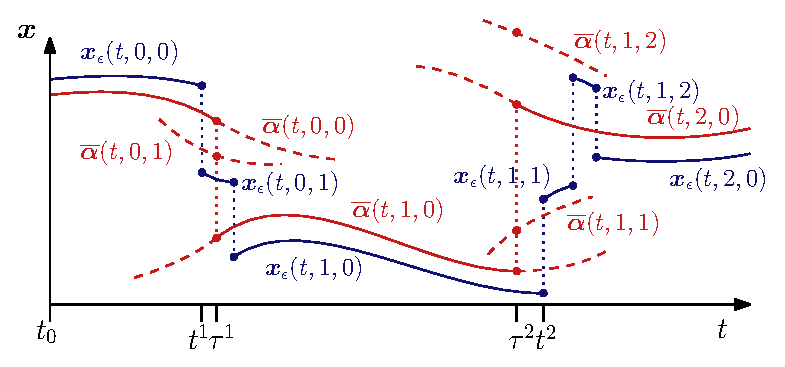
\includegraphics[width=.9\textwidth]{simulmicro.eps}\caption{The state evolution of the reference trajectory and state trajectory. The reference trajectory is enriched with phantom segments, to which the micro segments of the state trajectory can be compared.}\label{fig:4simulmicro}
\end{figure}

\nomenclature[Ri]{$i$}{The macro event counter}%
\nomenclature[Rk]{$k$}{The micro event counter}%
\nomenclature[Rc]{$c_i$}{The event-character of macro event $i$}%
\nomenclature[Rl]{$l_\kappa$}{The number of simultaneous activations of macro event $\kappa$}%
\nomenclature[Rs]{$s^k_i$}{The event-mode descriptor of macro event $i$ and micro event $k$}%
\nomenclature[RS]{$S^k_i$}{The historical notation of macro event $i$ from micro event $0$ up to $k$}%
\nomenclature[G07]{$\eta$}{The set of indexes of inactive guards}%
\nomenclature[Rt]{$t_i^k$}{The perturbed event time of micro event $k$ in macro event $i$}%

\section{Approximating perturbed trajectories with simultaneous events}
Using the notation presented in Section~\ref{sec:4not}, an approximation of the NSITHS will be derived for trajectories with simultaneous activations. First, a sensitivity analysis is presented for a simultaneous event with character 2. The result is used to define a jump gain that approximates the behavior of a simultaneous event with an arbitrary event-character, which holds for a particular sequence of events. Since multiple sequences of events are feasible in a simultaneous event, multiple jump gains can be associated with such an event. These jump gains are used to define a positively homogeneous jump gain, which is a state- and input-dependent jump gain that describes the jumping behavior of the state near ($\alphab,\mub$). Finally, the PTTHS is formally defined, which is a approximation of the NSITHS near the reference trajectory. Similar to the LTTHS presented in Section~\ref{sec:3approx}, we presume that the PTTHS is a first-order approximation of the NSITHS. The proof that the approximation is first order is not yet available, however.

\subsection{Sensitivity analysis for simultaneous guard-activation}
Similar to the sensitivity analysis for trajectories with isolated events presented in Section~\ref{sec:3sens}, the continuous macro segments ($k=0$) of the state trajectory can be approximated as
\begin{align}
\xb_i^\epsilon(t) = \bar{\alphab}_i + \epsilon\bar{\zb}_i + o(\epsilon),
\end{align}
where the subscript $(\cdot)^\epsilon$ indicates that the variable is dependent on $\epsilon$ and $\zb_i$ satisfies
\begin{align}
\dot{\zb}_i = \Ab_i(t)\zb_i +\Bb_i(t)\vb_i,\quad i\in \dom\alphab
\end{align}
with
\begin{align*}
\Ab_i(t) &= D_1\fb_i(\alphab_i,\mub_i,t),\\
\Bb_i(t) &= D_2\fb_i(\alphab_i,\mub_i,t).
\end{align*}
We will now derive an approximation of the jump map of a simultaneous event with character $c_i = 2$. A more thorough derivation can be found in Appendix~\ref{app:multjumps}. In this chapter, the macro counter $i$ is dropped for the sake of readability. By posing $\ls^{s^{k+1}}\gb := \ls^{s^{k+1}\leftarrow s^k}\gb$, the perturbed post-event state associated with micro event $k+1$ is given by
\begin{align}
\ls^{s^{k+1}}\xb^\epsilon(t^{k+1}) = \ls^{s^{k+1}}\gb(\ls^{s^{k}}\xb^\epsilon(t^{k+1}),\ls^{s^{k}}\ub^\epsilon(t^{k+1}),t^{k+1}),\label{eq:4xe012}
\end{align}
with
\begin{align}
\ls^{s^{k}}\xb^\epsilon(t^{k+1}) = \int_{t^{k}}^{t^{k+1}}\left[\ls^{s^{k}}\fb\left(\ls^{s^{k}}\xb^\epsilon(t),\ls^{s^{k}}\ub^\epsilon(t),t\right)\right]dt + \ls^{s^{k}}\gb\left(\ls^{s^{k-1}}\xb^\epsilon(t^{k}),\ls^{s^{k-1}}\ub^\epsilon(t^{k}),t^{k}\right).\label{eq:4xe01}
\end{align}
Here the left superscript $\ls^{s^k}(\cdot)$ indicates that the variable is in micro segment $k$ and $t^k$ represents the event-time of micro event $k$. Similar to \eqref{eq:3Delta}, we define the micro event time as
\begin{align}
\Delta^k := \left.\frac{\textnormal{d} t^k}{\textnormal{d}\epsilon}\right|_{\epsilon=0} = -\frac{D_1\ls^{s^{k}}\gamma\cdot\ls^{s^{k-1}}\bar{\zb}(\tau) + D_2\ls^{s^{k}}\gamma\cdot\ls^{s^{k-1}}\bar{\vb}(\tau)}{\ls^{s^{k}}\dot{\gamma}},\label{eq:4Deltak}
\end{align}
with
\begin{align*}
\ls^{s^k}\gamma &:= \ls^{s^k}\gamma(\ls^{s^{k-1}}\alphab(\tau),\ls^{s^{k-1}}\mub(\tau),\tau),\\
\ls^{s^k}\dot{\gamma} &:= D_1\ls^{s^{k}}\gamma\cdot\ls^{s^{k-1}}\fb + D_2\ls^{s^{k}}\gamma\cdot\ls^{s^{k-1}}\dot{\mub} + D_3\gamma^-.
\end{align*}
The right-hand side of \eqref{eq:4xe012} is expanded with respect to $\epsilon$, to find
\begin{align}
\ls^{s^{k+1}}\xb^\epsilon(t^{k+1}) = \ls^{s^{k+1}}\alphab(\tau) + \epsilon\left.\frac{\partial}{\partial\epsilon}\ls^{s^{k+1}}\gb\right|_{\epsilon=0} + o(\epsilon),\label{eq:4xe012exp}
\end{align}
where, similar to the expansion of $\gb_j(\xb^-,\ub^-,t_j)$ in \eqref{eq:3gexp},
\begin{multline}
\left.\frac{\partial\ls^{s^{k+1}}\gb}{\partial\epsilon}\right|_{\epsilon=0} = D_1\ls^{s^{k+1}}\gb\cdot\bigg(\ls^{s^k}\dot{\alphab}(\Delta^{k+1}-\Delta^{k}) + D_1\ls^{s^k}\gb\cdot\left(\ls^{s^{k-1}}\zb+\ls^{s^{k-1}}\dot{\alphab}\Delta^{k}\right) + D_2\ls^{s^k}\gb\cdot\left(\ls^{s^{k-1}}\vb+\ls^{s^{k-1}}\dot{\mub}\Delta^{k}\right) \\ + D_3\ls^{s^k}\gb\cdot\Delta^{k} \bigg)+ D_2 \ls^{s^{k+1}}\gb\cdot\left(\ls^{s^{k}}\vb+\ls^{s^{k}}\dot{\mub}\Delta^{k+1} \right) + D_3\ls^{s^{k+1}}\gb\cdot\Delta^{k+1},\label{eq:4dg1de}
\end{multline}
with
\begin{align*}
\ls^{s^k}\fb &:= \ls^{s^k}\fb(\ls^{s^{k}}\alphab(\tau),\ls^{s^{k}}\mub(\tau),\tau),\\
\ls^{s^k}\gb &:= \ls^{s^k}\gb(\ls^{s^{k-1}}\alphab(\tau),\ls^{s^{k-1}}\mub(\tau),\tau),\\
\ls^{s^k}\dot{\gb} &:= D_1\ls^{s^k}\gb\cdot \ls^{s^{k-1}}\fb + D_2\ls^{s^k}\gb\cdot \ls^{s^{k-1}}\dot{\mub} + D_3\ls^{s^k}\gb.
\end{align*}
In \eqref{eq:4dg1de}, the expansion of the post-event state $\ls^{s^{k+1}}\xb^\epsilon(t^{k+1})$ is expressed in terms of $\ls^{s^{k}}$ and $\ls^{s^{k-1}}$. This is done to find a relation between the ante-event state and input perturbation and the post-event state perturbation. By expanding the left-hand side of \eqref{eq:4xe012} with respect to $\epsilon$, we find
\begin{align}
\ls^{s^{k+1}}\xb^\epsilon(t^{k+1}) &= \ls^{s^{k+1}}\bar{\alphab}(t^{k+1})+\epsilon\ls^{s^{k+1}}\bar{\zb}(t^{k+1}) + o(\epsilon),\\
&= \ls^{s^{k+1}}\alphab(\tau) + \epsilon\ ^{s^{k+1}}\dot{\alphab}(\tau)\Delta^{k+1} + \epsilon\ ^{s^{k+1}}\zb(\tau) + o(\epsilon).\label{eq:4xexp}
\end{align}
From the work in Section~\ref{sec:3sens}, the jump gains $\Gb$ and $\Jb$ are derived for single events. With $\ls^{s^k}\Gb(t) := \ls^{s^{k}\leftarrow s^{k-1}}\Gb(t)$ and $\ls^{s^k}\Jb(t) := \ls^{s^{k}\leftarrow s^{k-1}}\Jb(t)$, these jump gains translate to the micro-event case as
\begin{align}
\ls^{s^k}\Gb(\tau) &= D_1\ls^{s^k}\gb - \left(\ls^{s^k}\dot{\gb} - \ls^{s^{k}}\fb\right)\frac{D_1\ls^{s^k}\gamma}{\ls^{s^k}\dot{\gamma}},\\
\ls^{s^k}\Jb(\tau) &= D_2\ls^{s^k}\gb - \left(\ls^{s^k}\dot{\gb} - \ls^{s^{k}}\fb\right)\frac{D_2\ls^{s^k}\gamma}{\ls^{s^k}\dot{\gamma}}.
\end{align}
Using \eqref{eq:4xe012exp} and \eqref{eq:4xexp}, an expression for $\ls^{s^{k+1}}\zb(\tau)$ is found, which is
\begin{multline}
\ls^{s^{k+1}}\zb(\tau) = D_1\ls^{s^{k+1}}\gb\cdot\ls^{s^{k}}\fb\Delta^{k+1} - D_1\ls^{s^{k+1}}\gb\cdot\ls^{s^{k}}\fb\Delta^{k} + D_1\ls^{s^{k+1}}\gb\cdot \bigg( D_1\ls^{s^{k}}\gb\cdot\left(\ls^{s^{k-1}}\zb+\ls^{s^{k-1}}\fb\Delta^{k}\right)\\
+D_2\ls^{s^{k}}\gb\cdot\left(\ls^{s^{k-1}}\vb+\ls^{s^{k-1}}\dot{\mub}\Delta^{k}\right)+D_3\ls^{s^{k}}\gb\cdot\Delta^{k}\bigg) + D_2 \ls^{s^{k+1}}\gb\cdot\left(\ls^{s^{k}}\vb+\ls^{s^{k}}\dot{\mub}\Delta^{k+1} \right) + \left(D_3\ls^{s^{k+1}}\gb - \ls^{s^{k+1}}\fb\right)\Delta^{k+1}.\label{eq:4ztau}
\end{multline}
which can be rewritten to 
\begin{multline}
\ls^{s^{k+1}}\zb(\tau) = \left(D_1\ls^{s^{k+1}}\gb - \left(D_1\ls^{s^{k+1}}\gb\cdot\ls^{s^{k}}\fb  + D_2\ls^{s^{k+1}}\gb\cdot\ls^{s^{k}}\dot{\mub} + D_3\ls^{s^{k+1}}\gb - \ls^{s^{k+1}}\fb\right)\frac{D_1\ls^{s^{k+1}}\gamma}{\ls^{s^{k+1}}\dot{\gamma}} \right)\ls^{s^k}\Gb\ls^{s^{k-1}}\zb\\
+ \left(D_1\ls^{s^{k+1}}\gb - \left(D_1\ls^{s^{k+1}}\gb\cdot\ls^{s^{k}}\fb  + D_2\ls^{s^{k+1}}\gb\cdot\ls^{s^{k}}\dot{\mub} + D_3\ls^{s^{k+1}}\gb - \ls^{s^{k+1}}\fb\right)\frac{D_1\ls^{s^{k+1}}\gamma}{\ls^{s^{k+1}}\dot{\gamma}} \right)\ls^{s^k}\Jb\ls^{s^{k-1}}\vb\\
+ \left(D_2\ls^{s^{k+1}}\gb - \left(D_1\ls^{s^{k+1}}\gb\cdot\ls^{s^{k}}\fb  + D_2\ls^{s^{k+1}}\gb\cdot\ls^{s^{k}}\dot{\mub} + D_3\ls^{s^{k+1}}\gb - \ls^{s^{k+1}}\fb\right)\frac{D_2\ls^{s^{k+1}}\gamma}{\ls^{s^{k+1}}\dot{\gamma}} \right)\ls^{s^{k}}\vb,
\end{multline}
which is equal to
\begin{align}
&\ls^{s^{k+1}}\zb(\tau) = \ls^{s^{k+1}}\Gb\ \ls^{s^{k}}\Gb\ \ls^{s^{k-1}}\zb + \ls^{s^{k+1}}\Gb\ \ls^{s^{k}}\Jb\ \ls^{s^{k-1}}\vb + \ls^{s^{k+1}}\Jb\ \ls^{s^{k}}\vb.\label{eq:4zkplusfinal}
\end{align}
An important realization is that \eqref{eq:4zkplusfinal} is also found by evaluating two single jumps at $\tau$, and taking the post-event state of the first jump as the ante-event state of the second jump. These two jumps are given by
\begin{align}
\ls^{s^{k}}\zb(\tau) &= \ls^{s^{k}}\Gb\ \ls^{s^{k-1}}\zb + \ls^{s^{k}}\Jb\ \ls^{s^{k-1}}\vb,\\
\ls^{s^{k+1}}\zb(\tau) &= \ls^{s^{k+1}}\Gb\ \ls^{s^{k}}\zb + \ls^{s^{k+1}}\Jb\ \ls^{s^{k}}\vb,
\end{align}
respectively. This implies that the approximation of the post-impact state of two simultaneous jumps at $\tau$ can be found by evaluating the two jumps separately. For an arbitrary number of micro events $k$, the approximation of the post-event state can be found to be
\begin{align}
\ls^{S^k}\zb(\tau) = \ls^{s^k\leftarrow s^0}\Gb\ \ls^{s^0}\zb(\tau) + \sum_{\iota=0}^{k-1}\ls^{s^{k}\leftarrow s^{\iota+1}}\Gb\ \ ^{s^{\iota+1}\leftarrow s^{\iota}}\Jb\ \ls^{s^{\iota}}\vb(\tau),\label{eq:4ljumps}
\end{align}
where $\ls^{p\leftarrow a}\Gb$ and $\ls^{p\leftarrow a}\Jb$ are defined as
\begin{align}
\ls^{p\leftarrow a}\Gb &:= \ls^{p}\Gb\ \ls^{p-1}\Gb\cdots\ls^{a}\Gb,\\
\ls^{p\leftarrow a}\Jb &:= \ls^{p}\Jb\ \ls^{p-1}\Jb\cdots\ls^{a}\Jb,
\end{align}
for a sequence $p\leftarrow p-1 \leftarrow \cdots \leftarrow a$, with slight abuse of notation, in the sense that $p-1$ indicates the mode descriptor associated to the mode before $p$. 
\begin{sloppypar}
\begin{myremark}
While it is not proven that \eqref{eq:4ljumps} is true, it is strongly suggested by the relation found in \eqref{eq:4zkplusfinal}. Whereas \eqref{eq:4zkplusfinal} only holds for a simultaneous event with character-2 ($c=2$), an induction-like proof can extend the derivation presented in this section to be true for an event with an arbitrary character, resulting in the relation given in \eqref{eq:4ljumps}. This proof, however, is left for future work.
\end{myremark}
\end{sloppypar}
The relation between the post-event state perturbation $\ls^{s^{k+1}}\zb(\tau)$ and the ante-event state and input perturbation $\ls^{s^{k-1}}\zb$ and $\vb$ in \eqref{eq:4ljumps} is the main result of this section. Using that result, the effect of a perturbation on the jumping behavior of the system can be approximated. For a more complete derivation, consult Appendix~\ref{app:multjumps}. The first term in \eqref{eq:4ljumps} represents the effect of the perturbed ante-event state on the perturbed post-event state. This term is already found in \cite{Rijnen2018}, where a sensitivity analysis is presented without input-dependent guards and jump maps. The summation in \eqref{eq:4ljumps} is a contribution of this work, which represents the effects of the chosen feedback during micro-segments.

Note that the approximation of the post-event state \eqref{eq:4ljumps} shares an algebraic similarity with the impulse response of linear discrete time systems. With $\xb_d(t)$ the state, $\ub_d(t)$ the input, and $\yb_d(t)$ the output of a discrete system, the discrete impulse response is in the form of
\begin{align}
\yb_d(t) = \Cb\xb_d(0) + \sum_{j=0}^t\Db(j)\ub_d(t-j),
\end{align}
where $\yb_d(t) :=  \yb_d(\xb_d(0),\ub(t),t)$, and $\Cb$ and $\Db$ some matrices defined by the discrete systems dynamics \cite{Hespanha2009}. Note that, similar to the discrete impulse response $\yb_d$, the post-event perturbation $\ls^{S^k}\zb$ is also dependent on the ante-event state perturbation $\ls^{s^0}\zb$, the entire evolution of the input $\ub$, and the time $t$, i.e., $\ls^{S^k}\zb(\tau) := \ls^{S^k}\zb(\ls^{s^0}\zb,\vb,\tau)$.

When $\vb$ is considered a feedback term that is turned off when the first micro event is detected, then the approximation of the post-event state perturbation can be simplified to
\begin{align}
\ls^{S^k}\zb(\tau) &= \ls^{S^k}\Lb \begin{bmatrix}
\ls^{s^0}\zb(\tau) \\ \ls^{s^0}\vb(\tau)
\end{bmatrix}, \text{ with }\ls^{S^k}\Lb = \begin{bmatrix}
\ls^{S^k}\Gb & \ls^{S^{k\leftarrow 1}}\Gb\ \ls^{S^{1\leftarrow 0}}\Jb
\end{bmatrix},\label{eq:4ljumpssimp}
\end{align}
since only the ante-event feedback term will be non-zero. The jump gain $\ls^{S^k}\Lb$ defined in \eqref{eq:4ljumpssimp} is defined for a particular order of guard activations. When considering a simultaneous event, different trajectories close to $(\alphab,\mub)$ can be associated to different sequences of guard-activations. Since the sensitivity analysis considers all trajectories close to $(\alphab,\mub)$, several sequences of guard-activations, and therefore several jumps gains as in \eqref{eq:4ljumpssimp}, can be associated with a simultaneous event. In the next section, the jump gain \eqref{eq:4ljumpssimp} associated to an a priori known mode sequence is used to define a state-dependent jump gain, which covers all possible mode sequences. 

Note that the description of the jump gain given in \eqref{eq:4ljumpssimp} is less complicated than jump gain \eqref{eq:4ljumps} for a micro event where feedback is nonzero. Since the micro events usually happen too rapidly to control on, feedback is often turned off when micro events are taking place. Therefore, only situations with zero feedback during micro events are considered in this work. Under these considerations the jump gain in \eqref{eq:4ljumpssimp} is used from here on to define $\ls^{S^k}\Lb$.

\subsection{The positively homogeneous jump map}
As mentioned in Section~\ref{sec:simguards}, an event with simultaneous guard activation will experience loss of simultaneity when perturbations are introduced. Due to the loss of simultaneity, the order of events is unknown. For that reason, one simultaneous event has several feasible event sequences associated with it. For there to be a finite amount of possibilities of event sequences, all sequences should be growing. A graph of growing mode sequences is illustrated for a character-3 event ($c=3$) in Figure~\ref{fig:4growingseq}, where the nodes represent the possible system modes and the edges represent the possible transitions. When the mode sequences are growing, the edges are unidirectional. Therefore a finite number of paths can be found from the ante-event mode described by $s = 000$ to the post-event mode described by $s = 111$. When the mode sequences are not growing, the edges are bidirectional. One can then travel both ways over each edge, resulting in an infinite number of possible mode sequences.

\begin{figure}[bt!]
\centering
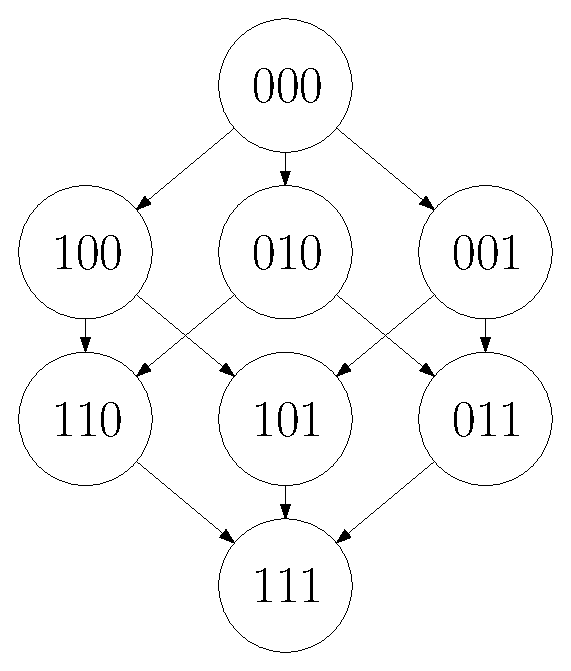
\includegraphics[width=.35\textwidth]{4growingseq.eps}\caption{An example of the possible modes in a character-3 event ($c=3$) illustrated with a graph. When the mode sequences are growing, the edges between the modes are unidirectional, resulting in a finite amount of paths to the post-event mode described by $s = 111$.}\label{fig:4growingseq}
\end{figure}

To be able to define a jump map, only a finite number of sequences can be considered. Therefore, an assumption is posed that the mode sequences should be growing.

\begin{sloppypar}
\begin{myass}[Growing mode sequences]\label{ass:unidirectional}
We assume, locally at each macro event, that all considered mode sequences are growing. Namely, at each micro event, all activated guards will remain active. In other words, considering one macro event, we assume that $s^0<s^1<\dots<s^l$, where $s^0= 00\dots0$ and $s^l = 11\dots1$, and $l$ is the number of micro events in the considered macro event.
\end{myass}
\end{sloppypar}

For example, when we consider a block with two contact points $\iota_1$ and $\iota_2$ executing a pushing motion towards a surface, with $s^0 = 00$ is both contact points open and $s^l = 11$ is both contact points in closed contact stick. Let us say we are in mode $s^1 = 10$, i.e., $\iota_1$ is in closed contact stick and $\iota_2$ is still open. The system goes through the second micro event by activating $\gamma^{01}_2$. Under Assumption~\ref{ass:unidirectional}, the event can not cause $\iota_1$ to release contact, i.e., $\Gamma_{\iota_1}^{\text{cl}\rightarrow\text{op}}>0$, $\Gamma_{\iota_1}^{\text{st}\rightarrow\text{sl}}>0$, $\gamma_{\iota_1}^{\text{cl}\rightarrow\text{op}}>0$ and $\gamma_{\iota_1}^{\text{st}\rightarrow\text{sl}}>0$ when solving the state reinitialization and mode selection presented in Section~\ref{sec:2discdyn}. Under Assumption~\ref{ass:unidirectional}, all mode sequences in a neighborhood of $\alphab,\mub$ will be growing and a finite number of jump gains are possible for a range of perturbations. Let us now pose an assumption on the association between guard functions and transitions.

\begin{sloppypar}
\begin{myass}[Guard-transition association]\label{ass:guardtrans}
We assume that activation of a guard will result in a transition associated with that guard, i.e., the guard function $\gamma^{\eta_k}$ activated in mode $s^{k-1}$, will result in a post-event mode of which the mode descriptor satisfies $s^{k} = s^{k-1} + \eta_k$. Here $\eta_k$ is the index of the guard function that is activated during micro event $k$.
\end{myass}
\end{sloppypar}

\begin{sloppypar}
\begin{myremark}
Considering mechanical systems, Assumption~\ref{ass:guardtrans} is easily verified for most guard functions. Because $\gamma^{\text{op}\rightarrow\text{cl}}_{\iota} = \hrm_{n,\iota}(\qb)$ is defined on position level, under Assumption~\ref{ass:unidirectional} it will always be contact point $\iota$ that will change mode when $\gamma^{\text{op}\rightarrow\text{cl}}_{\iota}$ is activated. For guard functions defined on acceleration level, i.e.,
\begin{align*}
\gamma^{\textnormal{st}\rightarrow\textnormal{sl}} &= \mu_\iota^2\lambda_{n,\iota} - \lambdab^T_{t,\iota}\lambdab_{t,\iota},\\
\gamma^{\textnormal{cl}\rightarrow\textnormal{op}} &= \lambda_{n,\iota},
\end{align*}
the situation is different. The feasible post-event mode is determined by the post-event acceleration for these guard functions. It is therefore possible that a guard function is activated in mode $s^{k-1}$, but is inactive in mode $s^{k}$. Under Assumption~\ref{ass:guardtrans} this is not possible. Therefore a constraint is introduced on the post-event acceleration, which can be determined by the set of equations, called the mode selection in Section~\ref{sec:2discdyn},
\begin{align}
\ddot{\qb}^+ &= \Mb^{-1}\left[\Sb\ub^+ - \Cb + \Wb_{n}\lambdab^+_{n} + \Wb_{t}\lambdab^+_{t}\right], &  \nonumber\\
\wb^T_{n,\iota}\ddot{\qb}^+ + \dot{\wb}^T_{n,\iota}\dot{\qb}^+ &= 0, & \forall \iota\in\Ic_{\text{cl}},\nonumber\\
\lambdab^+_{t,\iota}||\Wb_{t,\iota}^T\dot{\qb}^+|| + \mu\lambda^+_{n,\iota}\Wb_{t,\iota}^T\dot{\qb}^+ &= 0, & \forall \iota\in\Ic_{\text{sl}},\nonumber\\
\Wb^T_{t,\iota}\ddot{\qb}^+ + \dot{\Wb}^T_{t,\iota}\dot{\qb}^+ &= 0. & \forall \iota\in\Ic_{\text{st}},\nonumber
\end{align}
From the mode selection we can conclude that the post-event acceleration $\ddot{\qb}$ is directly dependent on the post-event input $\ub^+$. Therefore, the post-event input $\ub^+$ should be chosen in such a way that Assumption~\ref{ass:guardtrans} is met. Appendix~\ref{app:instantslip} gives an example of an event for which the guard is not necessarily associated with the transition the system goes through.
\end{myremark}
\end{sloppypar}
A state-dependent jump gain for all possible mode sequences associated to a simultaneous event will be defined in the following. This jump gain should consider all growing sequences that can take place for that range of perturbations. Therefore, a state-dependent matrix gain is defined, in the form of
\begin{align}
\ls^{p \leftarrow a}\Hb(\ls^{a}\zb(\tau),\ls^{a}\vb(\tau),\tau) = \left\lbrace\begin{array}{ll}
\Hb^1(\ls^{s^0}\zb,\ls^{s^0}\vb,\tau), & \text{if condition 1 is true},\\
\Hb^2(\ls^{s^0}\zb,\ls^{s^0}\vb,\tau), & \text{if condition 2 is true},\\
\vdots & \vdots\\
\Hb^{r}(\ls^{s^0}\zb,\ls^{s^0}\vb,\tau), & \text{if condition }r\text{ is true},
\end{array}\right.\label{eq:4Hgeneral}
\end{align}
where $r$ the number of possible mode sequences in a macro event. The jump map $\Hb$ is presented later in this section for a character-2 event ($c=2$). While it is possible to construct a straightforward algorithm that defines $\Hb$ for any character $c$, this is left as future work. We will now derive the jump maps and associated conditions in \eqref{eq:4Hgeneral} to obtain an explicit expression. Note that the several jump gains $\Hb$ in \eqref{eq:4Hgeneral} all coincide with a particular sequence of events.

For a certain perturbation, only a specific order of micro events is feasible. This order can be found by determining the perturbed jump time of all possible micro events, and selecting the micro event with the earliest event time as the next event. The perturbed event-time of the next micro event $\ls^{s^{k+1} \leftarrow S^{k}}t^\epsilon$ can be approximated at first order as
\begin{align}
t^{k+1} &= \tau + \epsilon\Delta^{k+1} + o(\epsilon),\\
&= \tau + \epsilon\left(\ls^{S^{k+1}}\ab^T\ \ls^{S^k}\zb +\ls^{S^{k+1}}\bb^T\ \ls^{S^k}\vb\right) + o(\epsilon),
\end{align}
with
\begin{align*}
\ls^{S^k}\ab &:= -\frac{1}{\dot{\gamma}^{\eta_k}}D_1\gamma^{\eta_k}(\ls^{s^{k-1}}\alphab,\ls^{s^{k-1}}\mub,\tau),\\
\ls^{S^k}\bb &:= -\frac{1}{\dot{\gamma}^{\eta_k}}D_2\gamma^{\eta_k}(\ls^{s^{k-1}}\alphab,\ls^{s^{k-1}}\mub,\tau).
\end{align*}
Defining the set mode descriptors related to all possible post-event modes 
\begin{align}
\mathcal{S} := \left\{ s^+ = s^- + \eta_+ \ |\ \eta_+\in \eta \right\},
\end{align}
the mode descriptor of the next mode can be written as
\nomenclature[RS]{$\mathcal{S}$}{The set of mode descriptors related to all possible post-event modes}%
\begin{align}
s^{k+1} = \underset{s^{\ast}}{\argmin}\left\{t^{k+1}\ |\ s^{\ast}\in\mathcal{S}\right\}.\label{eq:4argmin1}
\end{align}
Since the minimization of the impact-time does not depend on $\tau$ and $\epsilon$, we can rewrite \eqref{eq:4argmin1} to
\begin{align}
s^{k+1} = \underset{s^{\ast}}{\argmin}\left\{\ls^{S^{k+1}}\ab^T\ \ls^{S^k}\zb +\ls^{S^{k+1}}\bb^T\ \ls^{S^k}\vb\ |\ s^{\ast}\in\mathcal{S}\right\},
\end{align}
which can be written as
\begin{align}
s^{k+1} = s^k + \eta_{k+1},
\end{align}
with 
\begin{align}
\eta_{k+1} = \underset{\eta^\ast}{\argmin}\left\{-\frac{D_1\gamma^{\eta^\ast}(\ls^{s^k}\alphab,\ls^{s^k}\mub,\tau)\cdot\ls^{S^k}\zb + D_2\gamma^{\eta^\ast}(\ls^{s^k}\alphab,\ls^{s^k}\mub,\tau)\cdot\ls^{S^k}\vb}{\dot{\gamma}^{\eta^\ast}}\ \big|\ \eta^{\ast}\in\eta\right\}.\label{eq:4argmin2}
\end{align}
Here $\eta$ is the index set of inactive guard functions as defined in \eqref{eq:4eta} and $\eta_{k+1}$ is the identifier of the guard that is activated during micro event $k+1$. Finally, \eqref{eq:4argmin2} can be rewritten as
\begin{align}
\eta_{k+1} = \underset{\eta^*}{\argmin}\left(\ls^{S^\ast}\ab^T\ \ls^{S^k}\zb +\ls^{S^\ast}\bb^T\ \ls^{S^k}\vb\right),
\end{align}
with
\begin{align*}
\ls^{S^\ast}\ab &:= -\frac{1}{\dot{\gamma}^{\eta^\ast}}D_1\gamma^{\eta^\ast}(\ls^{s^k}\alphab,\ls^{s^k}\mub,\tau),\\
\ls^{S^\ast}\bb &:= -\frac{1}{\dot{\gamma}^{\eta^\ast}}D_2\gamma^{\eta^\ast}(\ls^{s^k}\alphab,\ls^{s^k}\mub,\tau).
\end{align*}
By checking \eqref{eq:4argmin2} for every micro event, we can determine what the post-event mode of each micro-event will be. With that knowledge, we can decide which jump gains we should apply in \eqref{eq:4ljumps} to find the correct jump gain.

We now pose an example to illustrate the positively homogeneous jump gain. Let us consider a system with $c_i = 2$, $\ls^{s^1}\vb=\ls^{s^2}\vb=\dots=\ls^{s^l}\vb=0$, and with a macro event starting in $s^0 = 00$ and ending in $s^l = 11$, this gives 
\begin{align}
\ls^{11\leftarrow 00}\Hb(\ls^{s^0}\zb(\tau),\ls^{s^0}\vb(\tau),\tau) = \left\lbrace\begin{array}{ll}
\begin{bmatrix}\ls^{11\leftarrow 00}_{\ls^{(12)}S^1}\Gb, & \ls^{11\leftarrow 00}_{\ls^{(12)}S^1}\Jb\end{bmatrix}, & \text{if }(\text{I}),\\
\begin{bmatrix}\ls^{11\leftarrow 01}_{\ls^{12}S^2}\Gb \ls^{01\leftarrow 00}_{\ls^{2}S^1}\Gb, & \ls^{11\leftarrow 01}_{\ls^{12}S^2}\Gb \ls^{01\leftarrow 00}_{\ls^{2}S^1}\Jb\end{bmatrix}, & \text{if }(\text{II}),\\
\begin{bmatrix}\ls^{11\leftarrow 10}_{\ls^{12}S^2}\Gb \ls^{10\leftarrow 00}_{\ls^{2}S^1}\Gb, & \ls^{11\leftarrow 10}_{\ls^{12}S^2}\Gb \ls^{10\leftarrow 00}_{\ls^{2}S^1}\Jb\end{bmatrix}, & \text{if }(\text{III}),
\end{array}\right.\label{eq:4H2200}
\end{align}
with
\begin{align}
(\text{I})&:\ls^{^2 S^1}\ab^T\ \ls^{s^0}\zb +\ls^{^2 S^1}\bb^T\ \ls^{s^0}\vb = \ls^{^1 S^1}\ab^T\ \ls^{s^0}\zb +\ls^{^1 S^1}\bb^T\ \ls^{s^0}\vb,\nonumber\\
(\text{II})&:\ls^{^2 S^1}\ab^T\ \ls^{s^0}\zb +\ls^{^2 S^1}\bb^T\ \ls^{s^0}\vb > \ls^{^1 S^1}\ab^T\ \ls^{s^0}\zb +\ls^{^1 S^1}\bb^T\ \ls^{s^0}\vb,\label{eq:4conds}\\
(\text{III})&:\ls^{^2 S^1}\ab^T\ \ls^{s^0}\zb +\ls^{^2 S^1}\bb^T\ \ls^{s^0}\vb < \ls^{^1 S^1}\ab^T\ \ls^{s^0}\zb +\ls^{^1 S^1}\bb^T\ \ls^{s^0}\vb.\nonumber
\end{align}

\begin{sloppypar}
\begin{myremark}
Note that the jump map \eqref{eq:4H2200} only applies to simultaneous activations in the same manifold. The situation where a single guard activation generates a post-event state that immediately activates another guard in the post-event mode is not what we name a simultaneous event. However, an example that might be worth exploring can be found in the application of this theory to mechanical systems. When a contact point impacts a surface, the post-event state of that event could immediately activate a stick/slip-transition related guard function. We believe that this situation might be worth exploring, because of its association with high performance. Let us consider a running robot. When it places one of his feet, it will want to push that foot as hard as possible while staying in stick. In this situation the reference trajectory might be chosen in such a way, that the post-event state of the impact is at the border of a stick-to-slip transition. We believe that a state-dependent matrix gain can be found, similar to \eqref{eq:4H2200}, which approximates the behavior of such events. This would be a useful addition to the RS control approach, and is therefore a suggestion for future research.
\end{myremark}
\end{sloppypar}

The jump gain in \eqref{eq:4H2200} is called a positively homogeneous jump gain for character-2 events ($c=2$). Due to the behavior of the simultaneous events, the linearity property of the jump gain is lost. This is shown in Appendix~\ref{app:poshom}. Instead, the jump gain is positively homogeneous, which is now formally defined.
 
\begin{sloppypar}
\begin{mydef}[Positive homogeneity]
Suppose that $\fb(\xb,\ub,t)$ is a continuously differentiable function. The function $\fb$ is positively homogeneous of degree $k$ in $\xb$ and $\ub$, and uniform in $t$, if 
\begin{align}
\fb(a\xb,a\ub,t) = a^k\fb(\xb,\ub,t),
\end{align}
for all $a>0$ \textnormal{\cite{Apostol1967}}.
\end{mydef}
\end{sloppypar}

The reader should be aware that the positively homogeneous jump gain \eqref{eq:4H2200} is non-unique. Due to the simultaneous activation of two guards $\gamma^{01}$ and $\gamma^{10}$, the term $\begin{bmatrix}\ls^{11\leftarrow 00}_{\ls^{(12)}S^1}\Gb, & \ls^{11\leftarrow 00}_{\ls^{(12)}S^1}\Jb\end{bmatrix}$ can be defined using either $\gamma^{01}$ or $\gamma^{10}$. However, this gain is only applied under the condition that 
\begin{align}
\ls^{^2 S^1}\ab^T\ \ls^{s^0}\zb +\ls^{^2 S^1}\bb^T\ \ls^{s^0}\vb = \ls^{^1 S^1}\ab^T\ \ls^{s^0}\zb +\ls^{^1 S^1}\bb^T\ \ls^{s^0}\vb,
\end{align}
which means that the positively homogeneous jump map $\ls^{11\leftarrow 00}\Hb\begin{bmatrix}\ls^{s^0}\zb & \ls^{s^0}\vb \end{bmatrix}^T$ is unique. For this reason, despite the jump gain $\ls^{11\leftarrow 00}\Hb$ being non-unique, the post-event state perturbation $\ls^{s^k}\zb$ resulting from the positively homogeneous jump gain is unique. 

The conditions that decide which jump gain to use are illustrated in Figure~\ref{fig:4cone}. Since the conditions are linear in $\zb$ and $\vb$, they appear as lines in the state space of $\zb$ and $\vb$. When we introduce more conditions, we will find several cones that relate a certain jump gain to a $\zb,\vb$ pair. When we look at the vector $\rb(\zb,\vb)$ in Figure~\ref{fig:4cone}, it can be noticed that when $\rb$ is multiplied with a positive constant $a$, the same jump gain is applied. Therefore, the positively homogeneous jump gain \eqref{eq:4H2200} is positively homogeneous of order zero. The non-uniqueness of $\ls^{11\leftarrow 00}\Hb$ appears on the dashed line associated with condition (I), depicted in Figure~\ref{fig:4cone}.

\begin{figure}[bt!]
\centering
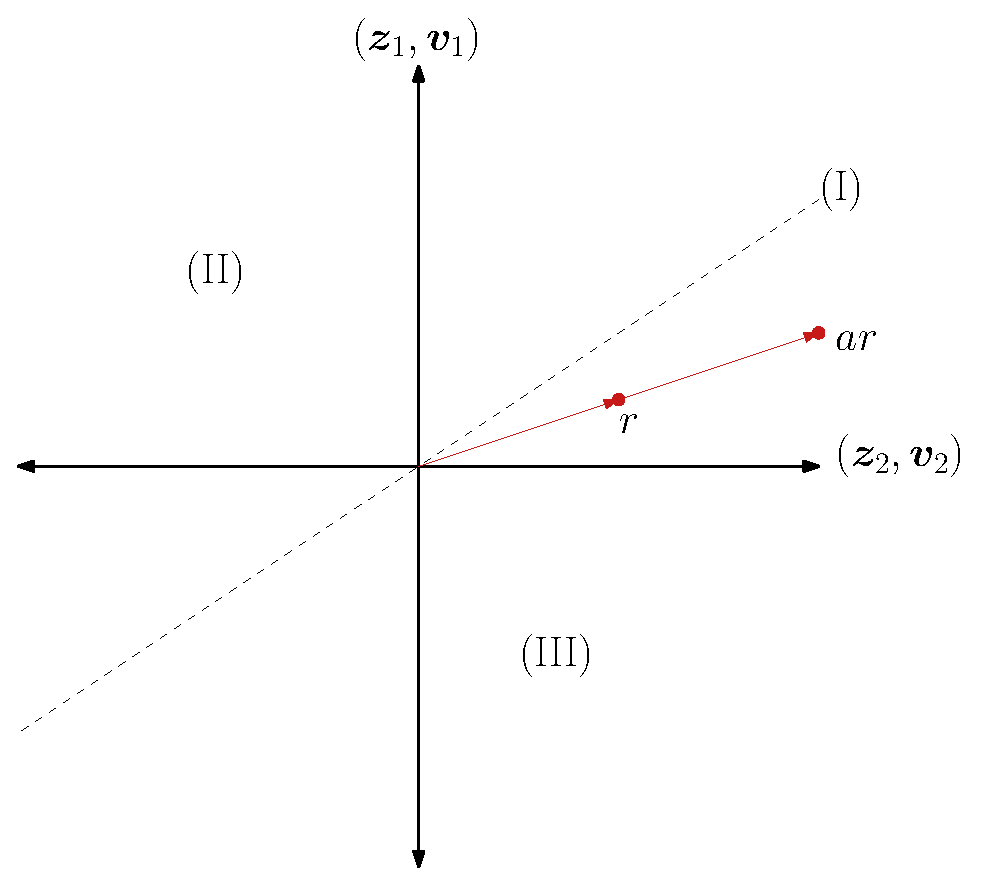
\includegraphics[width=.5\textwidth]{4cone.eps}\caption{An illustration of the conditions in \eqref{eq:4conds}, and how they result in a order zero positively homogeneous jump gain. The areas \textnormal{(I)}, \textnormal{(II)}, and \textnormal{(III)} coincide with the conditions \textnormal{(I)}, \textnormal{(II)}, and \textnormal{(III)} in \eqref{eq:4conds}.}\label{fig:4cone}
\end{figure}


\subsection{The positively homogeneous time-triggered hybrid system}\label{def:4PTTHS}
With the positively homogeneous jump gain presented in the previous section, the PTTHS can be defined. The PTTHS forms an approximation of the NSITHS defined in Definition~\ref{def:3nsiths}. We presume this approximation to be first order. The PTTHS will jump at the same time as the nominal trajectory $\alphab$, and will also experience the same number of jumps. This means that a controller designed on the PTTHS will only switch once during a macro event, and not on every micro event. This is desired behavior, as the micro events will likely happen too rapidly to control on. We now define the PTTHS formally, with the positively homogeneous jump gain being defined for a character-2 event ($c = 2$, with $a = 00$ and $p=11$) for brevity reasons.

\begin{sloppypar}
\begin{mydef}[PTTHS]
The positively homogeneous time-triggered hybrid system associated with the NSITHS and the associative and transversal reference trajectory ($\alphab(t,i),\mub(t,i)$) is given by
\begin{align}
\dot{\zb} &= \Ab_i(t)\zb + \Bb_i(t)\vb, &(t,i)&\in \dom\ \alphab,\\
\zb^+ &= \Hb_{i+1}\begin{bmatrix} \zb^- \\ \vb^-\end{bmatrix}, &(t,i)&\in \eve\ \alphab,
\end{align}
where $\Hb_{i+1} := \ls^{p\leftarrow a}\Hb(\zb^-,\vb^-,t)$ is a positively homogeneous jump gain of order zero,
\begin{align*}
\Ab_i(t) &:= D_1\fb(\alphab(t,i),\mub(t,i),t,i),\\
\Bb_i(t) &:= D_2\fb(\alphab(t,i),\mub(t,i),t,i),\\
\vb^- &:= \ls^{a}\vb = \vb(t,i),\\
\zb^- &:= \ls^{a}\zb = \zb(t,i),\\
\zb^+ &:= \ls^{p}\zb = \zb(t,i+1),
\end{align*}
with $a = s_i^0 = 00\dots0$ and $p = s_i^l = 11\dots1$ where $l$ is the amount of micro events in the growing sequence $p\leftarrow\dots\leftarrow a$. The domain $\dom\ \alphab$ and event set $\eve\ \alphab$ are defined as
\begin{align}
\dom\ \alphab &:= \bigcup_{i=0}^N[\tau_i,\tau_{i+1}]\times \{i\},\\
\eve\ \alphab &:= \bigcup_{i=1}^N\{\tau_i\}\times \{i-1\},
\end{align}
with $\tau_0 = t_0$. The positively homogeneous jump gain $\ls^{p\leftarrow a}\Hb$ for a character-2 event ($c=2$), with the macro counter $i$ omitted for readability, is given by
\begin{align}
\ls^{11\leftarrow 00}\Hb(\ls^{s^0}\zb(\tau),\ls^{s^0}\vb(\tau),\tau) = \left\lbrace\begin{array}{ll}
\begin{bmatrix}\ls^{11\leftarrow 00}_{\ls^{(12)}S^1}\Gb, & \ls^{11\leftarrow 00}_{\ls^{(12)}S^1}\Jb\end{bmatrix}, & \text{if }(\textnormal{I}),\\
\begin{bmatrix}\ls^{11\leftarrow 01}_{\ls^{12}S^2}\Gb \ls^{01\leftarrow 00}_{\ls^{2}S^1}\Gb, & \ls^{11\leftarrow 01}_{\ls^{12}S^2}\Gb \ls^{01\leftarrow 00}_{\ls^{2}S^1}\Jb\end{bmatrix}, & \text{if }(\textnormal{II}),\\
\begin{bmatrix}\ls^{11\leftarrow 10}_{\ls^{12}S^2}\Gb \ls^{10\leftarrow 00}_{\ls^{2}S^1}\Gb, & \ls^{11\leftarrow 10}_{\ls^{12}S^2}\Gb \ls^{10\leftarrow 00}_{\ls^{2}S^1}\Jb\end{bmatrix}, & \text{if }(\textnormal{III}),
\end{array}\right.\label{eq:4PTTHS1}
\end{align}
with
\begin{align}
(\text{I})&:\ls^{^2 S^1}\ab^T\ \ls^{s^0}\zb +\ls^{^2 S^1}\bb^T\ \ls^{s^0}\vb = \ls^{^1 S^1}\ab^T\ \ls^{s^0}\zb +\ls^{^1 S^1}\bb^T\ \ls^{s^0}\vb,\nonumber\\
(\text{II})&:\ls^{^2 S^1}\ab^T\ \ls^{s^0}\zb +\ls^{^2 S^1}\bb^T\ \ls^{s^0}\vb > \ls^{^1 S^1}\ab^T\ \ls^{s^0}\zb +\ls^{^1 S^1}\bb^T\ \ls^{s^0}\vb,\label{eq:4PTTHS2}\\
(\text{III})&:\ls^{^2 S^1}\ab^T\ \ls^{s^0}\zb +\ls^{^2 S^1}\bb^T\ \ls^{s^0}\vb < \ls^{^1 S^1}\ab^T\ \ls^{s^0}\zb +\ls^{^1 S^1}\bb^T\ \ls^{s^0}\vb.\nonumber
\end{align}
The jump gains $\ls^{s^+\leftarrow s^-}_{S^k}\Gb$ and $\ls^{s^+\leftarrow s^-}_{S^k}\Jb$ in \eqref{eq:4PTTHS1}, with $s^+ = s^k$ and $s^- = s^0$ and $S^k = s^k\leftarrow s^{k-1} \leftarrow \cdots \leftarrow s^0$, are given by
\begin{align}
\ls^{s^+\leftarrow s^-}_{S^k}\Gb &:= D_1\gb^- - \left(\dot{\gb}^- - \fb^+\right)\frac{D_1\gamma^-}{\dot{\gamma}^-},\\
\ls^{s^+\leftarrow s^-}_{S^k}\Jb &:= D_2\gb^- - \left(\dot{\gb}^- - \fb^+\right)\frac{D_2\gamma^-}{\dot{\gamma}^-},
\end{align}
and
\begin{align*}
\fb^- &:= \ls^{s^-}\fb\left(\ls^{S^-}\alphab(\tau),\ls^{S^-}_{\rightarrow}\mub(\tau),\tau\right),\\
\fb^+ &:= \ls^{s^+}\fb\left(\ls^{S^+}\alphab(\tau),\ls^{S^+}_{\rightarrow}\mub(\tau),\tau\right),\\
\gb^- &:= \ls^{s^+\leftarrow s^-}\gb\left(\ls^{S^-}\alphab(\tau),\ls^{S^-}_{\rightarrow}\mub(\tau),\tau\right),\\
\gamma^- &:= \gamma^{\eta(s^+\leftarrow s^-)}\left(\ls^{S^-}\alphab(\tau),\ls^{S^-}_{\rightarrow}\mub(\tau),\tau\right),\\
\dot{\gb}^- &:= D_1\gb^-\cdot \fb^- + D_2\gb^-\cdot \dot{\mub}^- + D_3\gb^-,\\
\dot{\gamma}^- &:= D_1\gamma^-\cdot\fb^- + D_2\gamma^-\cdot\dot{\mub}^- + D_3\gamma^-,
\end{align*}
where the $\rightarrow$ left subscript should be interpreted as $\searrow$ or $\nearrow$ to indicate whether the feedforward is pushing or withdrawing, respectively. $\gamma^{\eta(s^+\leftarrow s^-)}$ is the guard function that is activated during the transition $s^+\leftarrow s^-$. If the transition $s^+\leftarrow s^-$ is associated with multiple guard functions, one of the guard functions can be chosen, as it will have no effect on the jump gain. For example, during the transition $11\leftarrow 00$, $\gamma^{01}$ or $\gamma^{10}$ should be used for defined the jump gain. Finally, the vectors $\ls^{S^k}\ab$ and $\ls^{S^k}\bb$ in \eqref{eq:4PTTHS2} are given by
\begin{align*}
\ls^{S^k}\ab &= -\frac{1}{\dot{\gamma}^{-}}D_1\gamma^{-},\\
\ls^{S^k}\bb &= -\frac{1}{\dot{\gamma}^{-}}D_2\gamma^{-}.
\end{align*}
\end{mydef}
\end{sloppypar}

%\begin{figure}[h!]
%\centering
%\begin{subfigure}[b]{0.47\textwidth}   
%\centering 
%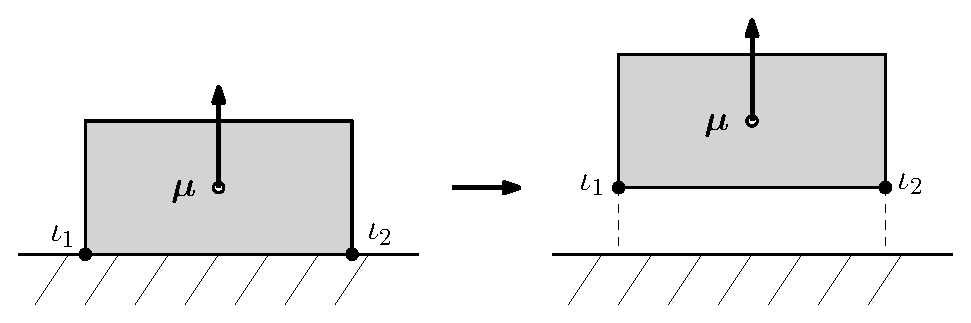
\includegraphics[width=\textwidth]{4example12.eps}
%\label{fig:4example1}\caption{The modes in the nominal trajectory.}
%\end{subfigure}
%\vskip\baselineskip
%\begin{subfigure}[b]{0.81\textwidth}   
%\centering 
%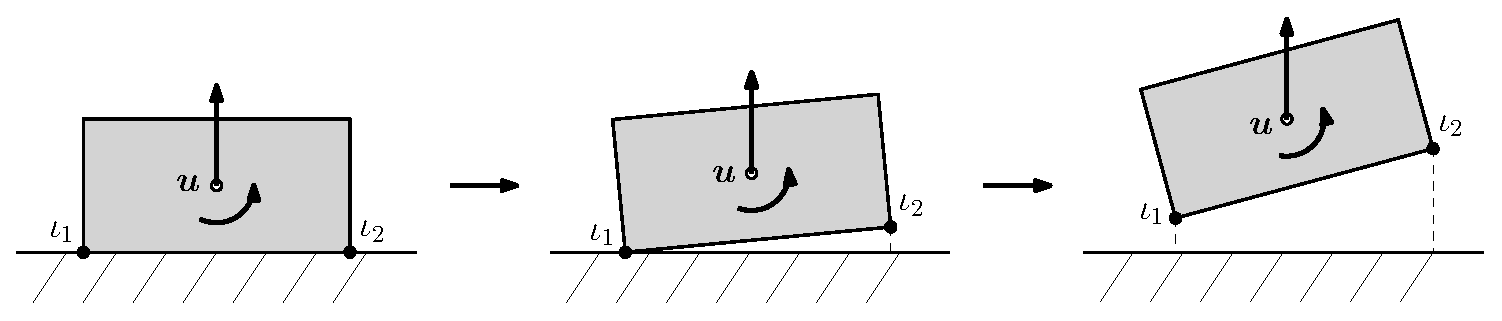
\includegraphics[width=\textwidth]{4example456.eps}
%\label{fig:4example4}\caption{The modes in a perturbed trajectory.}
%\end{subfigure}
%\vskip\baselineskip
%\begin{subfigure}[b]{\textwidth}   
%\centering 
%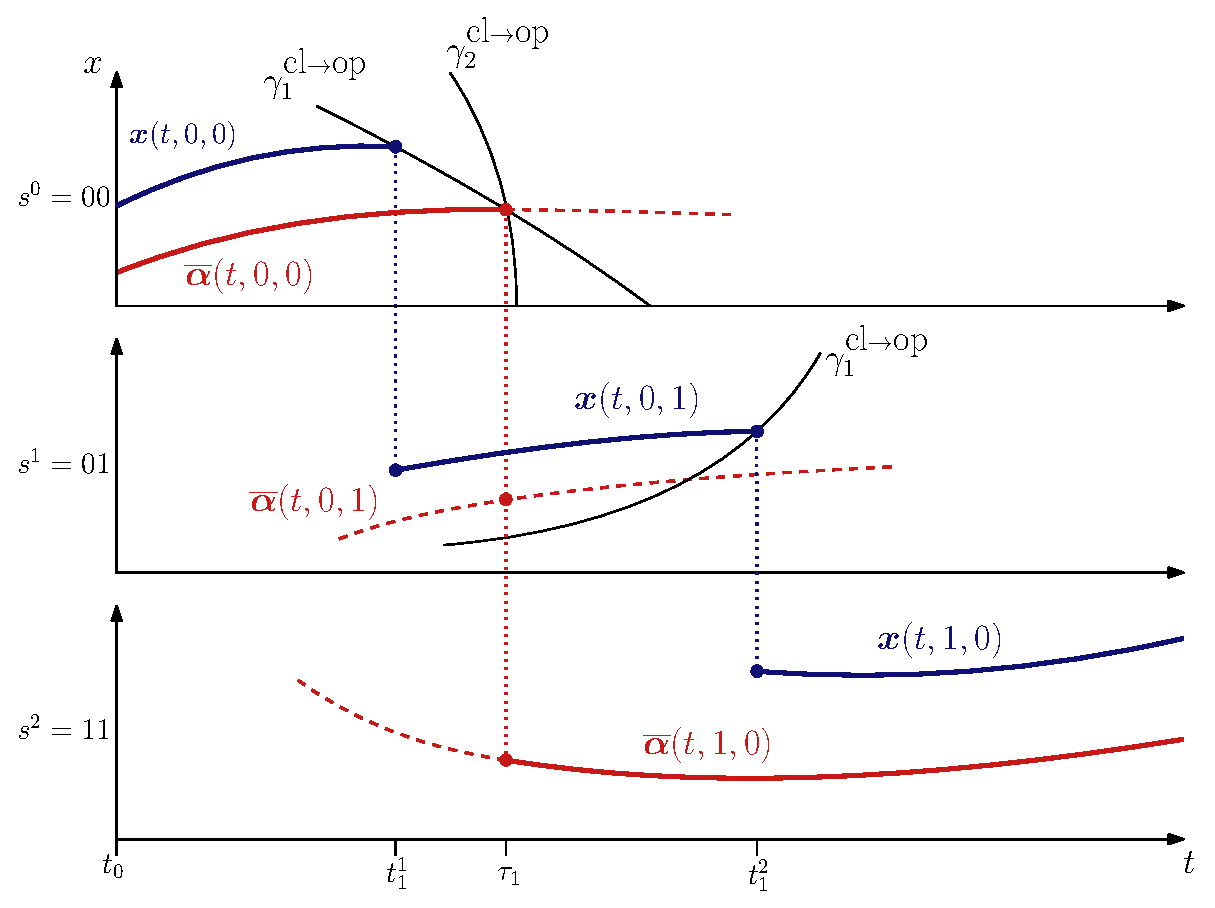
\includegraphics[width=.85\textwidth]{4exampletraj.eps}
%\label{fig:4exampletraj}
%\end{subfigure}
%\caption{The state evolution of the nominal and state trajectory is illustrated in this figure. }
%\label{fig:4example}
%\end{figure}

\nomenclature[RH]{$\Hb$}{The positively homogeneous jump gain}%
\nomenclature[Rz]{$\zb$}{The state perturbation}%
\nomenclature[Rv]{$\vb$}{The input perturbation}%
\nomenclature[RA]{$\Ab$}{Linear state matrix}%
\nomenclature[RB]{$\Bb$}{Linear input matrix}%
\nomenclature[A]{PTTHS}{Positively homogeneous Time-Triggered Hybrid System}%

\section{Summary}
An approximation for nonlinear state-and-input-triggered systems with input-dependent guard experiencing simultaneous impacts is presented. Simultaneous guard activations are introduced and the adopted notation required to deal with such activations is presented and elaborated. Assumptions on the reference trajectory are presented, which reduce the complexity of the problem while maintaining practical usability. Then, reference spreading is extended to transitions with simultaneous events. After that, a sensitivity analysis is presented, to find an approximation of the behavior of the NSITHS near ($\alphab,\mub$), where so-called loss of simultaneity occurs. Similar to the result presented in Chapter~\ref{ch:order}, we presume the approximation being first order, despite the proof not yet being available. A state-and-input dependent jump gain, called the positively homogeneous jump gain, is used to define the positively homogeneous time-triggered hybrid system (PTTHS). The PTTHS is expected to be suitable for assessing the local asymptotic stability of a nonlinear state-and-input triggered hybrid system with simultaneous guard activations.
\end{document}